\documentclass{article}

\usepackage{amsthm}
\usepackage{amsfonts}
\usepackage{amsmath}
\usepackage{amssymb}
\usepackage{fullpage}
\usepackage{float}

\usepackage{graphicx}

\usepackage[usenames]{color}
\usepackage{hyperref}
  \hypersetup{
    colorlinks = true,
    urlcolor = blue,       % color of external links using \href
    linkcolor= blue,       % color of internal links 
    citecolor= blue,       % color of links to bibliography
    filecolor= blue,        % color of file links
    }
    
\usepackage{listings}

\definecolor{dkgreen}{rgb}{0,0.6,0}
\definecolor{gray}{rgb}{0.5,0.5,0.5}
\definecolor{mauve}{rgb}{0.58,0,0.82}

\lstset{frame=tb,
  language=haskell,
  aboveskip=3mm,
  belowskip=3mm,
  showstringspaces=false,
  columns=flexible,
  basicstyle={\small\ttfamily},
  numbers=none,
  numberstyle=\tiny\color{gray},
  keywordstyle=\color{blue},
  commentstyle=\color{dkgreen},
  stringstyle=\color{mauve},
  breaklines=true,
  breakatwhitespace=true,
  tabsize=3
}

\theoremstyle{theorem} 
   \newtheorem{theorem}{Theorem}[section]
   \newtheorem{corollary}[theorem]{Corollary}
   \newtheorem{lemma}[theorem]{Lemma}
   \newtheorem{proposition}[theorem]{Proposition}
\theoremstyle{definition}
   \newtheorem{definition}[theorem]{Definition}
   \newtheorem{example}[theorem]{Example}
\theoremstyle{remark}    
  \newtheorem{remark}[theorem]{Remark}


\title{Programming Languages Report}
\author{Evelyn Lawrie\\ Chapman University}

\date{\today}

\begin{document}

\maketitle

\begin{abstract}
This report is composed of weekly homework assignments for the Programming Languages course at Chapman University. First, an introduction describes the objectives and contents of this report. Then, further sections explore each assigned problem, week by week. The report ends in a conclusion that summarizes the goals of this project and the larger context it belongs to. 
\end{abstract}

\tableofcontents

\section{Introduction}\label{intro}

This report's goal is to encourage problem solving and original thinking through the implementation of several self-contained weekly homework assignments. The task entails implementing a solution to each problem in a programming language of choice and then working out a given example of the algorithm's logic. By thinking through and thoroughly understanding each step of the algorithm, a deeper understanding of the logic behind why algorithms work the way that they do is cultivated. 

\section{Week 1}

\subsection{GCD Introduction}

The greatest common divisor algorithm can be understood from a geometric, algebraic, and programming perspective. The basis of this algorithm is the idea that whatever divides two numbers n and m where n \textgreater \text{} m must also divide n - m. This can be explored geometrically by visualizing small rectangles dividing up bigger rectangles until there is no smaller common divisor that will evenly fit in rectangles. This algorithm is also referred to as Euclid's algorithm, stemming from the Greek mathematician known as the ``father of geometry" \cite{Gcd}.

When exploring how algebra can solve the greatest common divisor problem, this entails breaking up the problem into three cases: 

\begin{itemize}
\item n \textgreater \text{} m
\item n \textless \text{} m
\item n = m
\end{itemize}

Here is the algebraic definition of Euclid's algorithm using the three cases as described above \cite{Ltx}: 

\begin{equation}
gcd (n, m) = 
\left\{
    \begin{array}{lr}
        gcd(m, m - n), & \text{if } n \text{ } \textgreater \text{ } m\\
        gcd(n, n - m), & \text{if } n \text{ } \textless \text{ } m\\
        n, & \text{if } n = m
    \end{array}
\right\}
\end{equation}

\subsection{GCD Code}

Below is a recursive implementation of the GCD function in Java. 

\begin{lstlisting}
// recursive function to implement the greatest common divisor of two integers
int gcdCalc(int n, int m) {
        if (n > m) {
            return gcdCalc(m, n - m); // subtract m from n when n is bigger 
        }
        else if (n < m) {
            return gcdCalc(n, m - n); // subtract n from m when m is bigger
        }
        else {
            return n; // return n when m and n are equal 
        }
    }
\end{lstlisting}

\subsection{Example Computation}

Below is an implementation of the greatest common divisor algorithm using the example numbers 9 and 33:

\begin{align}
gcd(9, 33) & = gcd(9, 33-9)\\
& = gcd(9, 24)\\
& = gcd(9, 24-9)\\
& = gcd(9, 15)\\
& = gcd(9, 15-9)\\
& = gcd(9, 6)\\
& = gcd(9-6, 6)\\
& = gcd(3, 6)\\
& = gcd(3, 6-3)\\
& = gcd(3, 3)\\
& = 3
\end{align}

\subsection{GCD Conclusion}

Recursion is the basis for many of these weekly assignments and is introduced in this first week. Understanding in detail how recursion works behind the scenes aids in the implementation of the coded solutions in this report. Recursion is a problem-solving technique that utilizes the call stack to create functions that call other functions, or more simplified versions of themselves, within them. To visualize and fully understand the structure of recursive calls, it is best to draw out the problem as a tree data structure, with each recursive call being a node of the tree. Every time a base case is reached, that node becomes a leaf and then the branches are explored upwards from there, branching off when needed and computing calculations from the bottom up. This is describing depth-first search, in which one branch of the tree is explored all the way until reaching a base case. This process is repeated for the whole tree, usually starting at the left and moving right. Parsing, rewriting strings into trees, is a method of visualizing how a computer executes a certain computation and can be vital in the comprehension of the recursion problems explored in this report. 

Another key takeaway from this week that improves upon the concept of recursion is memoization. This deals with the repeated nodes or function calls within a function's tree. With simple recursion, it is common for the same calculation to be computed multiple times, which decreases efficiency of the code. This creates exponential run times which can prove highly costly for large computations. The process of memoization stores values that the function has already computed in a hash table or similar data structure for easy lookup and avoidance of unnecessary repeated calculations. The recursive function call then implements a quick lookup in this data structure (constant runtime) and extracts the output if the current input value has already been calculated. If the current parameter has not been calculated, it performs the regular calculations and then stores the new value inside of the memo object. The process of memoization greatly decreases the time complexity of recursive functions, in the majority of cases bringing it down from an exponential to a polynomial or linear type runtime. This problem-solving technique stood out to me as a highly important lecture topic that serves as a way to optimize the algorithms presented in this report.

\section{Week 2}

\subsection{Towers of Hanoi Introduction}

Towers of Hanoi is a mathematical game in which disks are stacked in ascending order on the far left of three rods. The aim of this puzzle is to move these disks to the far right rod. For each move of one rod at a time, the rule must be obeyed that no disk can be placed onto a disk that is smaller than itself \cite{Wik}. The minimal number of moves required to find a solution given n number of disks is $2^n - 1$ \cite{Wik}.

In the calculation below, \textit{hanoi n x y} is describing a function call to move n disks from rod x to rod y. The far right rod is denoted with a 0, the middle as 1, and the right with a 2. This problem can be approached through recursion, with the function defined as: 

\begin{align}
hanoi \text{ }1 \text{ }x \text{ }y &=  move \text{ }x \text{ }y
\end{align}
\begin{align}
hanoi (n + 1) \text{ }x \text{ }y &=
hanoi \text{ }n \text{ }x \text{ }(other \text{ }x \text{ }y)\\
& move \text{ }x \text{ }y\\
& hanoi \text{ }n \text{ }(other \text{ }x \text{ }y) \text{ }y
\end{align}

The function \textit{move x y} is a function that takes the top disk from position x and moves it to position y. The term \textit{other x y} is the third rod, neither x nor y.

\subsection{Example Computation}

Below are the calculations of the hanoi function with the example of 5 rings moving from left to right: 

\begin{lstlisting}
hanoi 5 0 2  
    hanoi 4 0 1 
        hanoi 3 0 2
            hanoi 2 0 1 
                hanoi 1 0 2 = move 0 2 
                move  0 1
                hanoi 1 2 1 = move 2 1
            move 0 2  
            hanoi 2 1 2
                hanoi 1 1 0 = move 1 0  
                move  1 2  
                hanoi 1 0 2 = move 0 2
        move 0 1
        hanoi 3 2 1
            hanoi 2 2 0 
                hanoi 1 2 1 = move 2 1
                move 2 0
                hanoi 1 1 0 = move 1 0
            move 2 1 
            hanoi 2 0 1 
                hanoi 1 0 2 = move 0 2
                move 0 1
                hanoi 1 2 1 = move 2 1 
    move 0 2 
    hanoi 4 1 2 
        hanoi 3 1 0
            hanoi 2 1 2 
                hanoi 1 1 0 = move 1 0
                move 1 2
                hanoi 1 0 2 = move 0 2 
            move 1 0
            hanoi 2 2 0
                hanoi 1 2 1 = move 2 1
                move 2 0
                hanoi 1 1 0 = move 1 0
        move 1 2
        hanoi 3 0 2 
            hanoi 2 0 1
                hanoi 1 0 2 = move 0 2
                move 0 1
                hanoi 1 2 1 = move 2 1
            move 0 2
            hanoi 2 1 2
                hanoi 1 1 0 = move 1 0
                move 1 2
                hanoi 1 0 2 = move 0 2
\end{lstlisting}

Here are the 31 moves present in the above calculation:

\begin{enumerate}
  \centering
  \item move 0 2
  \item move 0 1
  \item move 2 1
  \item move 0 2
  \item move 1 0
  \item move 1 2
  \item move 0 2
  \item move 0 1
  \item move 2 1
  \item move 2 0
  \item move 1 0
  \item move 2 1
  \item move 0 2
  \item move 0 1
  \item move 2 1
  \item move 0 2
  \item move 1 0
  \item move 1 2
  \item move 0 2
  \item move 1 0
  \item move 2 1
  \item move 2 0
  \item move 1 0
  \item move 1 2
  \item move 0 2
  \item move 0 1
  \item move 2 1
  \item move 0 2
  \item move 1 0
  \item move 1 2
  \item move 0 2
\end{enumerate}

\subsection{Towers of Hanoi Formula}

The word \textit{hanoi} appears 31 times in the computation above. This is the same frequency as the number of moves per n amount of disks. Therefore, the formula for amount of function calls necessary for the computation of a given number of disks is: 


\begin{align}
numFunctionCalls(numDisks) = numMoves(numDisks) = 2^{numDisks} - 1
\end{align}

\subsection{Towers of Hanoi Conclusion}

The syntax that displays the example computation is designed to illustrate how the stack grows and shrinks with recursive function calls. The stack grows from left to right until a base case is reached, shrinking from there going right to left. Working through this example thoughtfully can aide in the understanding of how recursive functions are interacted with on the stack. We are able to visualize through the Towers of Hanoi problem what the call stack looks like behind the scenes and why recursive functions work the way that they do. Recursion is the basis for many of the computations explored throughout this course, making a thorough understanding of its implementation crucial in fully absorbing its key takeaways. 

\section{Week 3}

\subsection{Parsing Introduction}

Concrete syntax is defined as written code while abstract syntax is the representation of code, which is what the code means to the machine. Abstract syntax can be visualized with trees, and it is made up of algebraic/recursive data types. Parsing is the process of translating concrete syntax into abstract syntax. Some programming languages skip the parsing step and are composed of abstract syntax rather than concrete syntax. Parsing analyzes symbols using a parser generator to see whether they follow formal grammar rules, like the ones outlined by BNFC or other formal grammar structures. 

\subsection{Concrete Syntax Trees}

Given the context-free grammar: 

\begin{lstlisting}
Exp -> Exp '+' Exp1 
Exp1 -> Exp1 '*' Exp2              
Exp2 -> Integer            
Exp2 -> '(' Exp ')'  
Exp -> Exp1             
Exp1 -> Exp2 
\end{lstlisting}

The task is to implement concrete syntax trees for the example strings given. The grammar above is a set of rules that defines a language. In this case, that language is the set of arithmetic expressions using times and plus. Below are the written out parse trees:

\begin{figure}[H]
\begin{center}
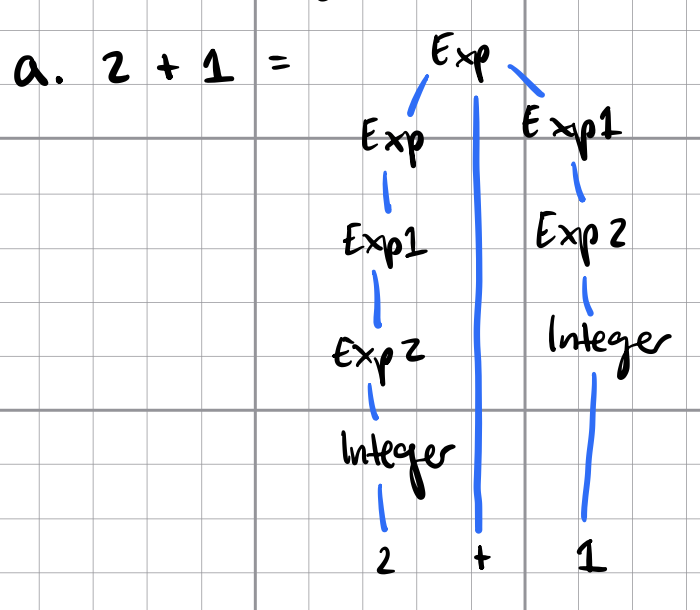
\includegraphics[scale=0.4]{img/C1.png}
\end{center}
\caption{2 + 1}\label{C1}
\end{figure}

\begin{figure}[H]
\begin{center}
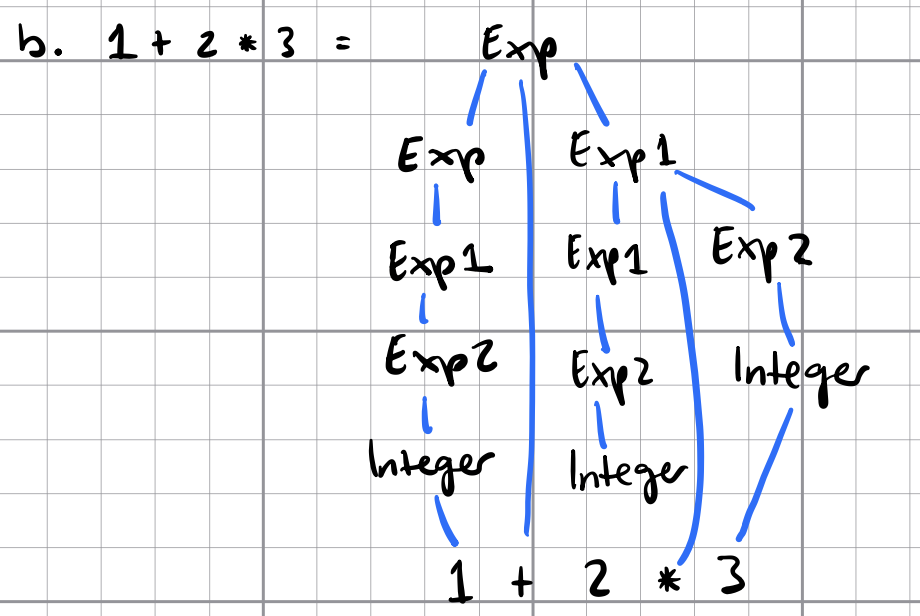
\includegraphics[scale=0.4]{img/C2.png}
\end{center}
\caption{1 + 2 * 3}\label{C2}
\end{figure}

\begin{figure}[H]
\begin{center}
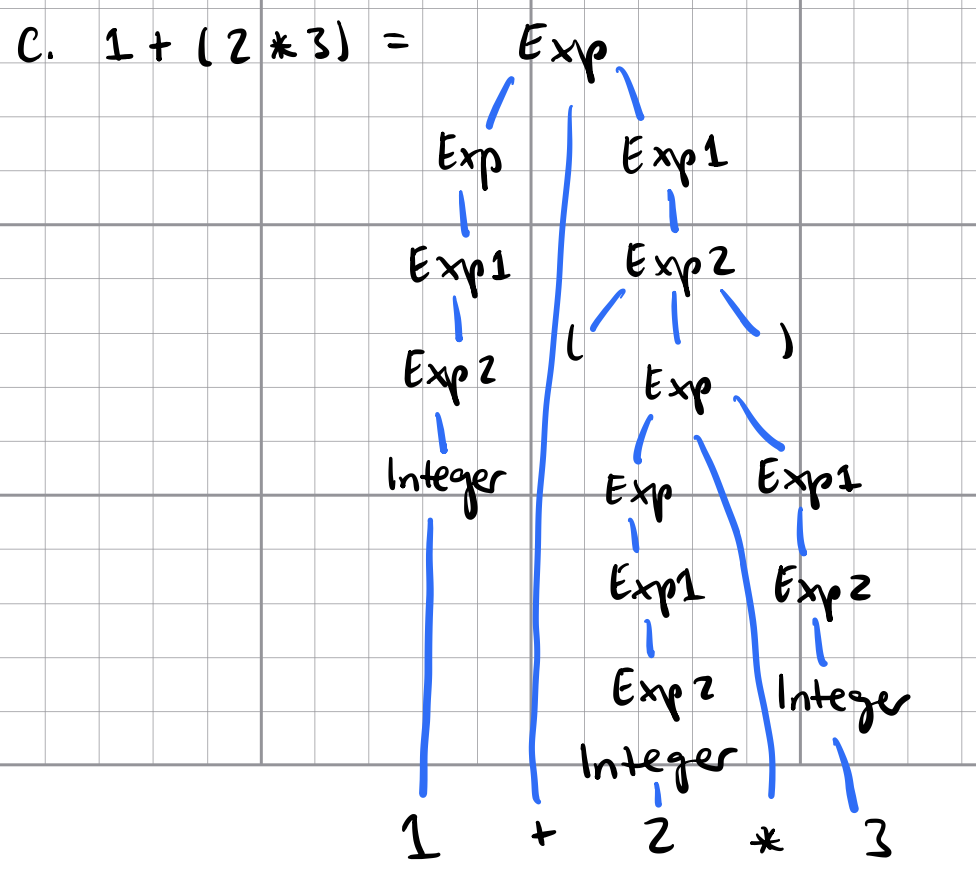
\includegraphics[scale=0.4]{img/C3.png}
\end{center}
\caption{1 + (2 * 3)}\label{C3}
\end{figure}

\begin{figure}[H]
\begin{center}
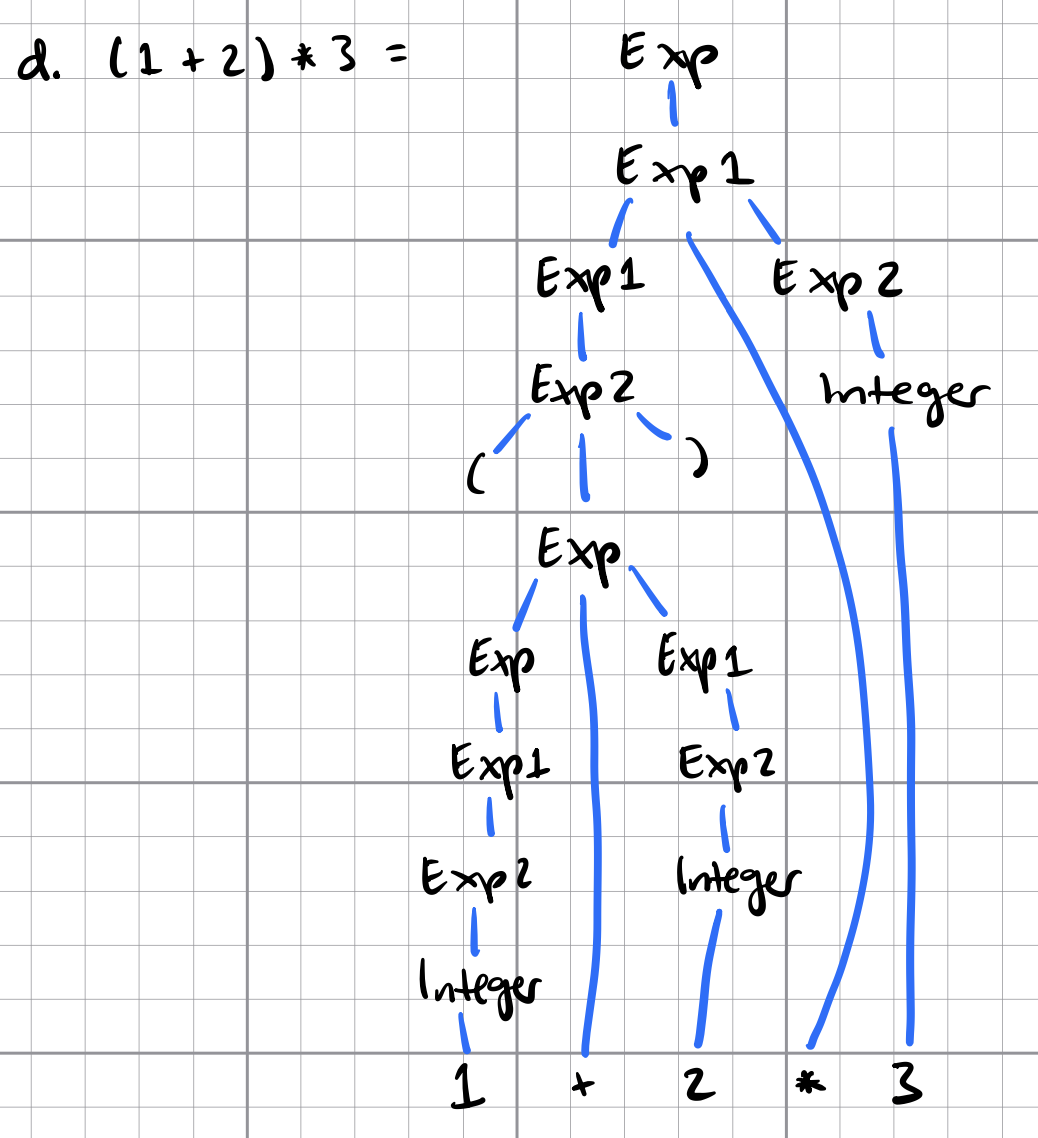
\includegraphics[scale=0.4]{img/C4.png}
\end{center}
\caption{(1 + 2) * 3}\label{C4}
\end{figure}

\begin{figure}[H]
\begin{center}
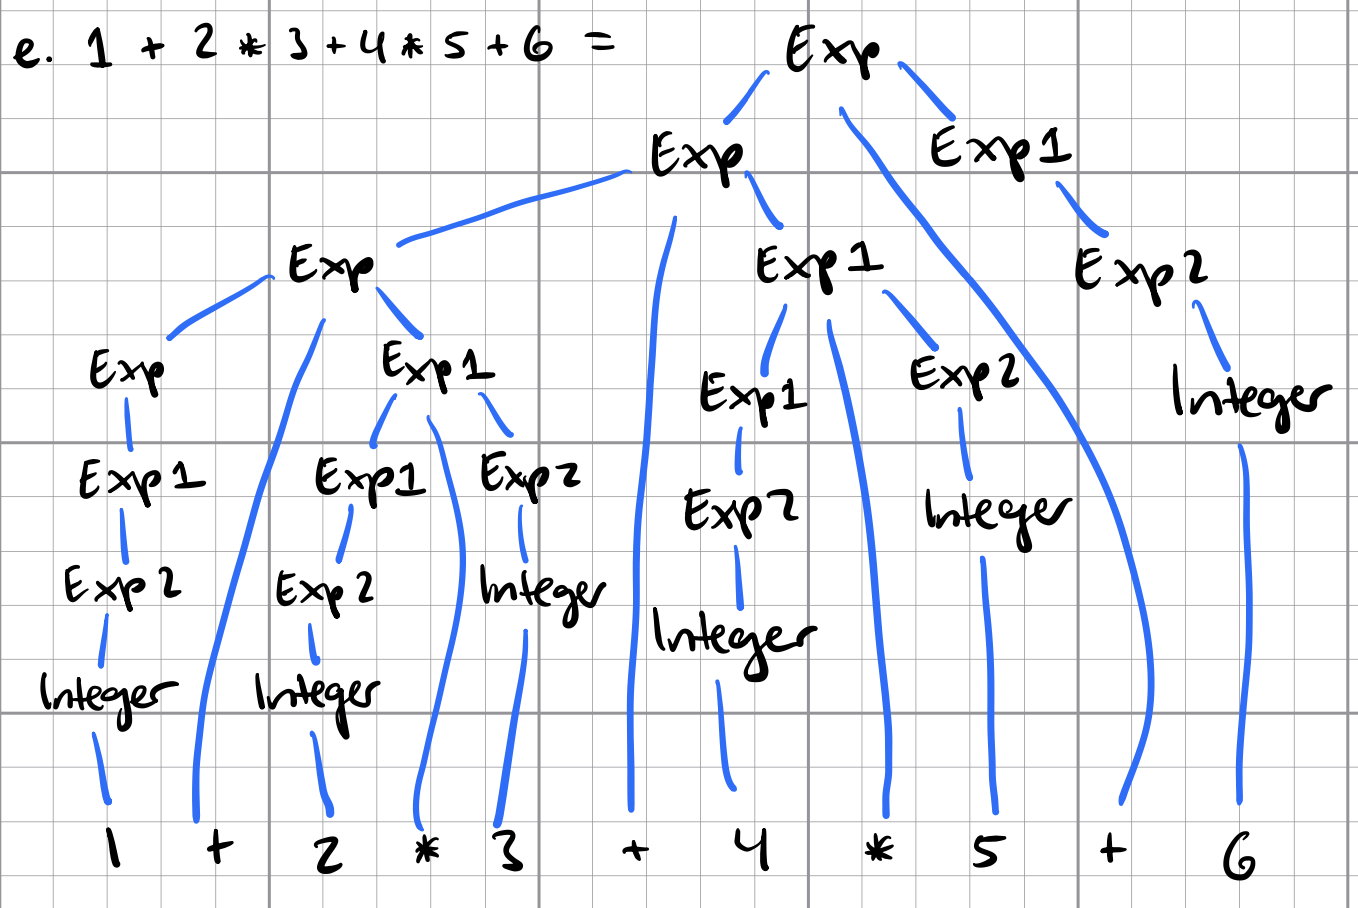
\includegraphics[scale=0.4]{img/C5.png}
\end{center}
\caption{1 + 2 * 3 + 4 * 5 + 6}\label{C5}
\end{figure}

\subsection{Abstract Syntax Trees}

Given the BNFC grammar: 

\begin{lstlisting}
Plus.   Exp ::= Exp "+" Exp1 ;
Times.  Exp1 ::= Exp1 "*" Exp2 ;
Num.    Exp2 ::= Integer ;
	
coercions Exp 2 ;
\end{lstlisting}

We are tasked with writing out the abstract syntax trees for the example arithmetic equations that follow the rules of the BNFC grammar defined above. BNFC comes with its own language, LNBF, which is a language for writing context-free grammars. The above set of rules is an example of what grammar looks like in BNFC and it represents the structure for the set of arithmetic equations that use plus and times. The following trees are written as abstract syntax trees. These trees differ from concrete syntax trees in three ways: the unnamed rules are eliminated, parent nodes are labeled with the names of the corresponding rules, and concrete syntax (such as symbols like "+" or "*") are eliminated. 

\begin{figure}[H]
\begin{center}
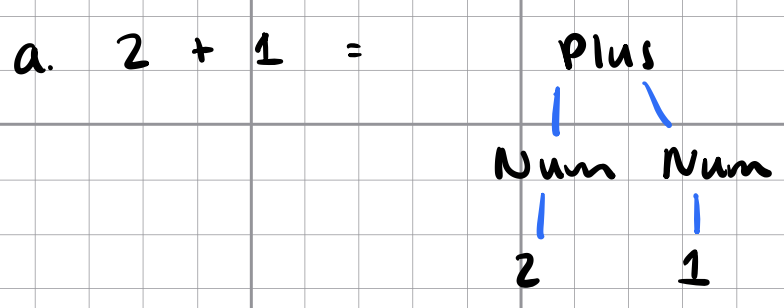
\includegraphics[scale=0.4]{img/A1.png}
\end{center}
\caption{2 + 1}\label{A1}
\end{figure}

\begin{figure}[H]
\begin{center}
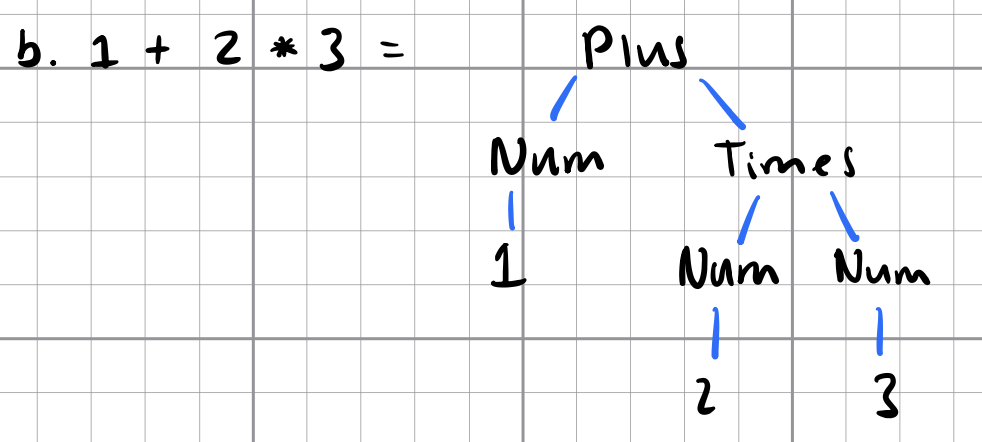
\includegraphics[scale=0.4]{img/A2.png}
\end{center}
\caption{1 + 2 * 3}\label{A2}
\end{figure}

\begin{figure}[H]
\begin{center}
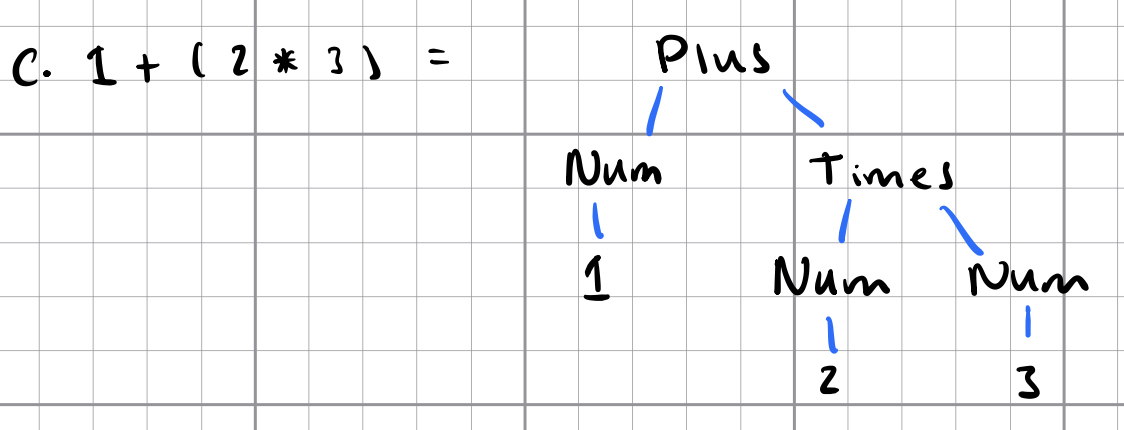
\includegraphics[scale=0.4]{img/A3.png}
\end{center}
\caption{1 + (2 * 3)}\label{A3}
\end{figure}

\begin{figure}[H]
\begin{center}
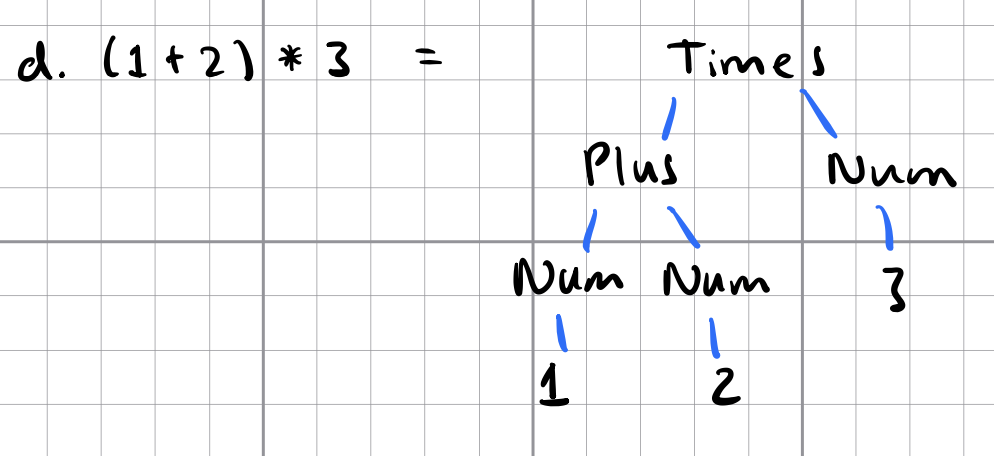
\includegraphics[scale=0.4]{img/A4.png}
\end{center}
\caption{(1 + 2) * 3}\label{A4}
\end{figure}

\begin{figure}[H]
\begin{center}
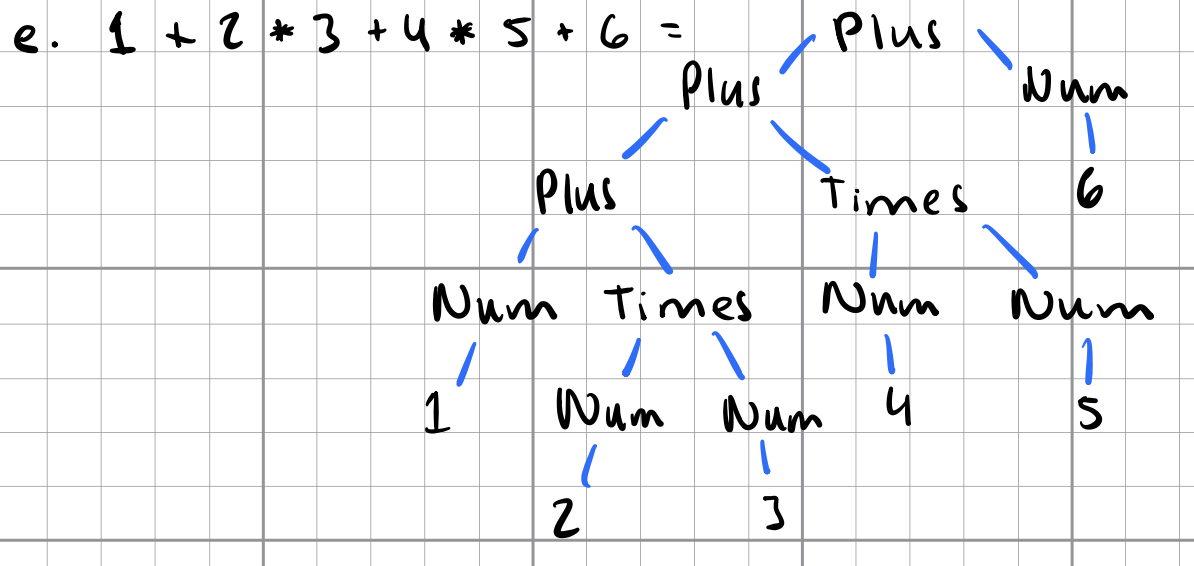
\includegraphics[scale=0.4]{img/A5.png}
\end{center}
\caption{1 + 2 * 3 + 4 * 5 + 6}\label{A5}
\end{figure}

Since parenthesis are not taken into account when writing out the nodes of abstract syntax trees, the tree for the equation $1+2*3$ is identical to the one for the equation $1+(2*3)$. The first equation follows the order of operations, in which multiplication is evaluated before addition. The second tree puts parenthesis around the multiplication terms, which visually illustrates which part of the equation to evaluate first, even though the equation is evaluated the same without the parenthesis given the order of operations. $(1+2)*3$ manipulates the order of operations, causing the addition to be evaluated first and therefore diverging from the calculation of the first equation without any parenthesis. 

\subsection{Parsing Conclusion}

Parsing is an important topic in this class, as it is an essential process that machines employ when evaluating most computer code. Computers parse concrete syntax into abstract syntax, which is then evaluated by the virtual machine, using the model of computation. This process is something we will encounter daily as computer programmers. Better understanding how a computer parses and understands the information we give it can make us more efficient programmers. Being able to decipher parse trees given a context-free grammar and examples of its language allows us to better understand how computers process code. BNFC and other types of parser generators define rules that the computer follows when interpreting concrete syntax strings. Approaching computer programs in terms of language and grammar teaches us to interpret programs logically and think of parsing as something that follows strict rules and does not take semantics into account. The way humans read and interpret programs is very different from how computers parse them, and we as programmers have to keep in mind that what the computer sees is taken at face value and evaluated according to the rules we have defined. This teaches us to be explicit and straightforward with how we program, avoiding ambiguity and confusion.

\section{Week 4}

\subsection{Lambda Calculus Introduction}

Lambda calculus only has three programming constructs. These are abstraction, application, and variables. According to abstraction, a program called $e$ containing the variable $x$ will look like $\lambda x. e$ in Lambda calculus. Application outlines how if $e1$ and $e2$ are programs, $e1 e2$  is the program that applies the function $e1$ to argument $e2$. Finally, the most basic programs in Lambda calculus only consist of variables. Lambda calculus abstracts away a lot of the syntax used in most other programming languages. The report this week focuses on the syntax and semantics of Lambda calculus.

\subsection{Syntax}

For the syntax portion of this week's homework, we are tasked with using the grammar of BNFC outlined for Lambda calculus to output the linearized abstract syntax trees from the following expressions, as well as manually write out the abstract syntax trees for them. Below are the calculations for the given Lambda calculus expressions: 

\begin{figure}[H]
\begin{center}
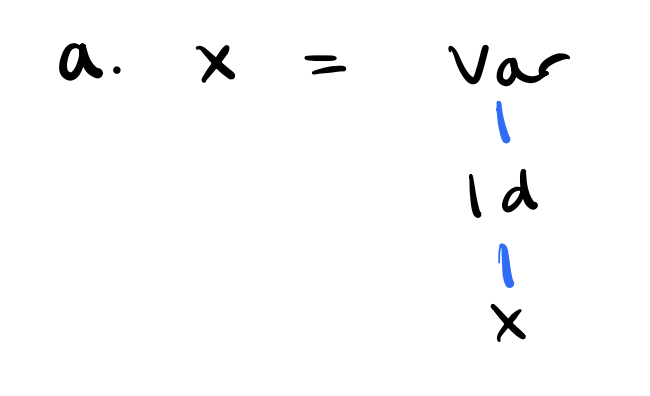
\includegraphics[scale=0.4]{img/aAST.png}
\\
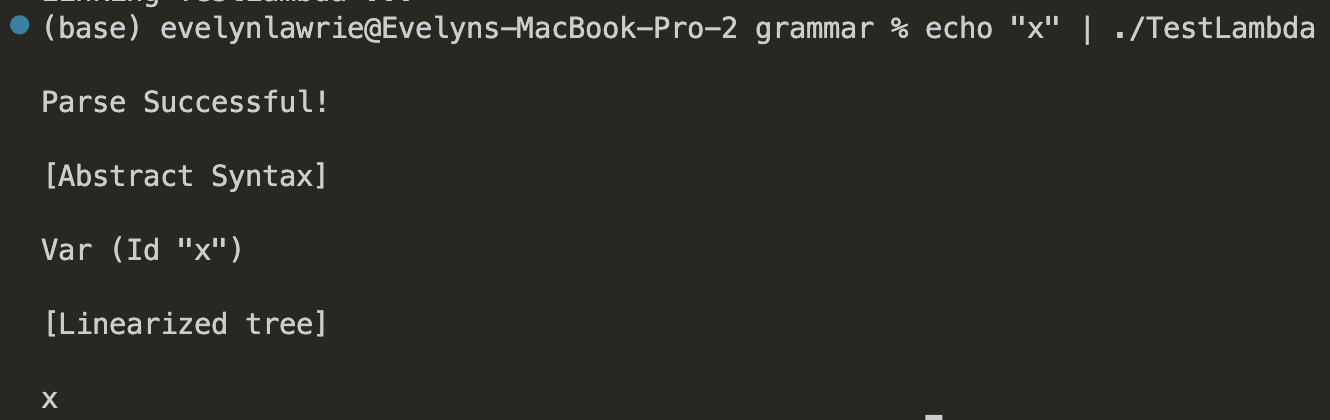
\includegraphics[scale=0.4]{img/ASTa.png}
\end{center}
\caption{x}\label{ASTa}
\end{figure}

\begin{figure}[H]
\begin{center}
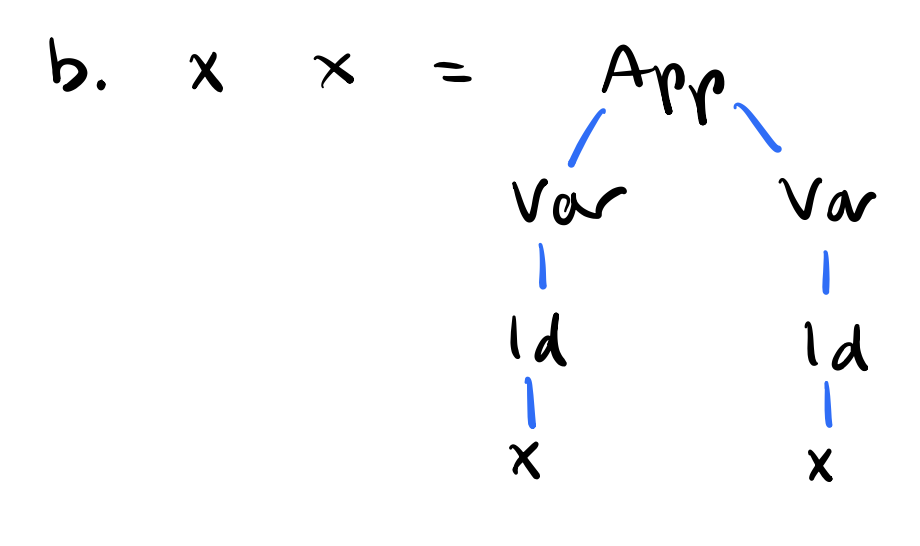
\includegraphics[scale=0.4]{img/bAST.png}
\\
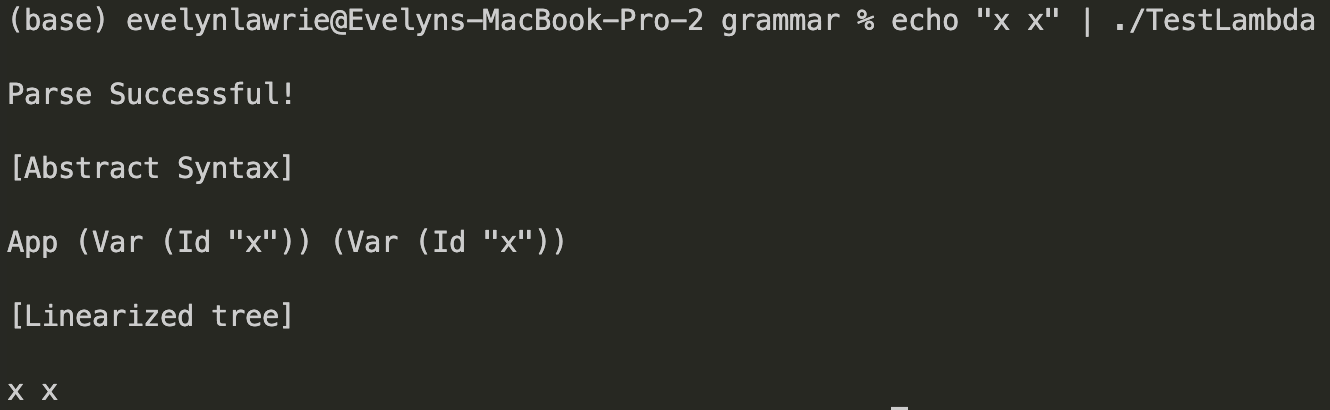
\includegraphics[scale=0.4]{img/ASTb.png}
\end{center}
\caption{x x}\label{ASTb}
\end{figure}

\begin{figure}[H]
\begin{center}
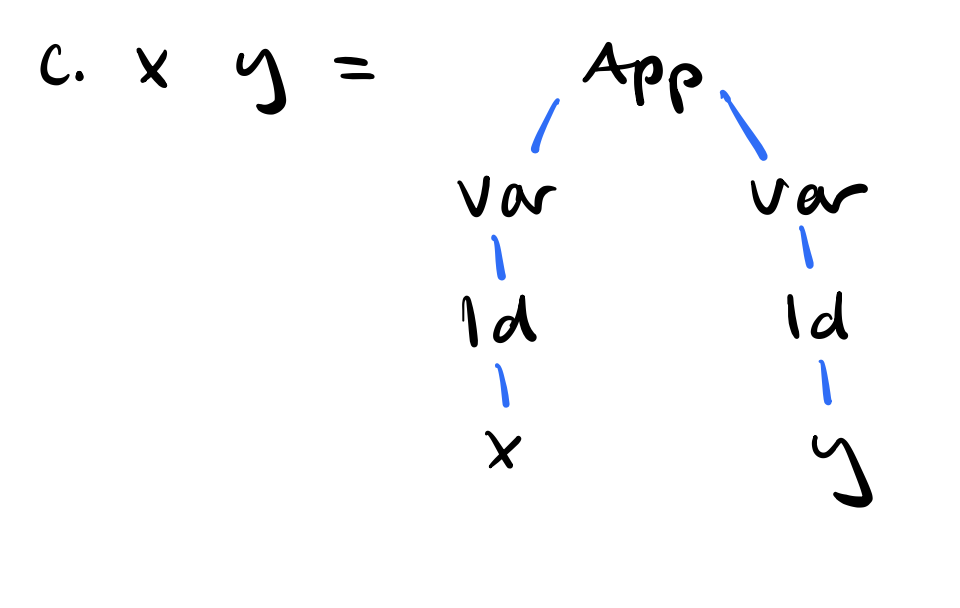
\includegraphics[scale=0.4]{img/cAST.png}
\\
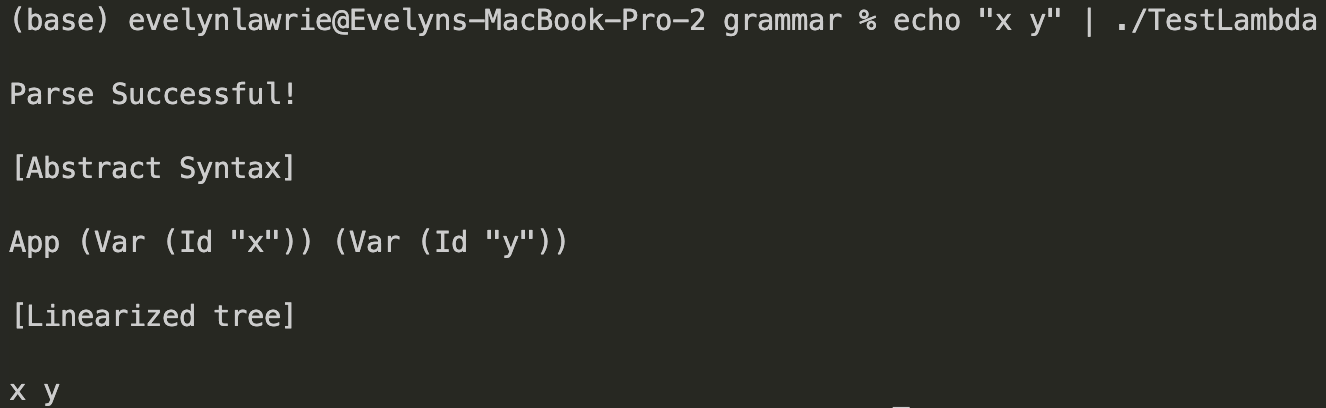
\includegraphics[scale=0.4]{img/ASTc.png}
\end{center}
\caption{x y}\label{ASTc}
\end{figure}

\begin{figure}[H]
\begin{center}
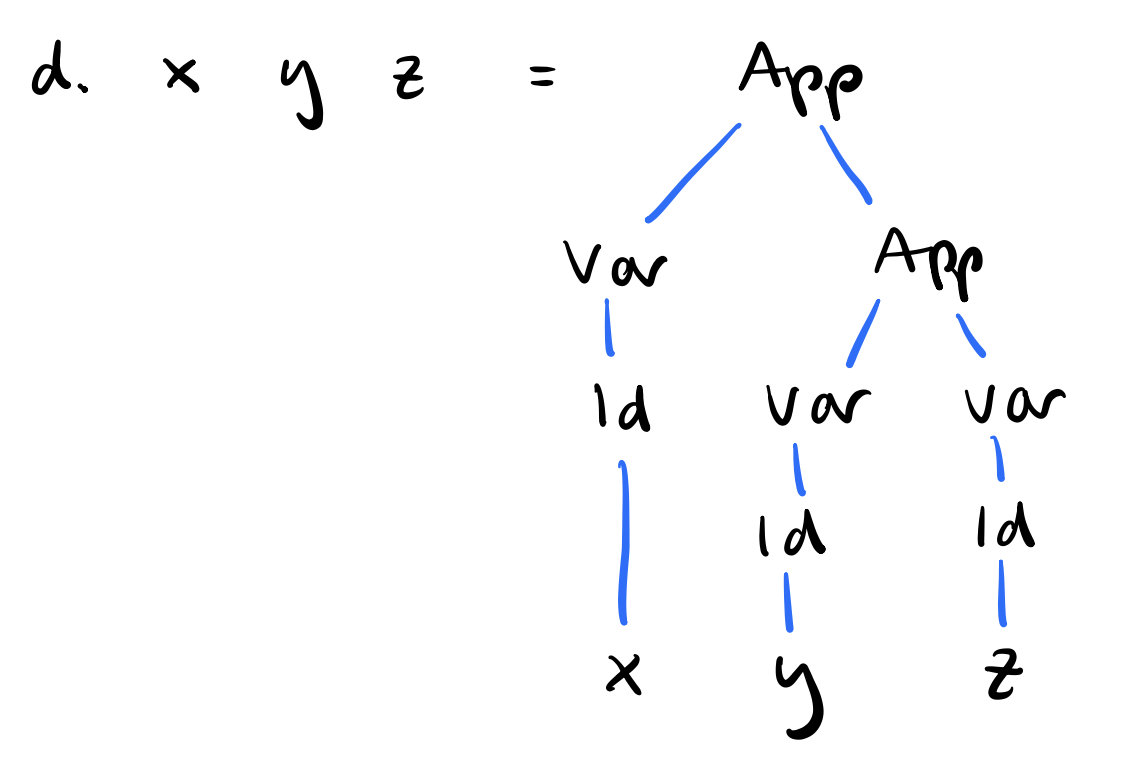
\includegraphics[scale=0.4]{img/dAST.png}
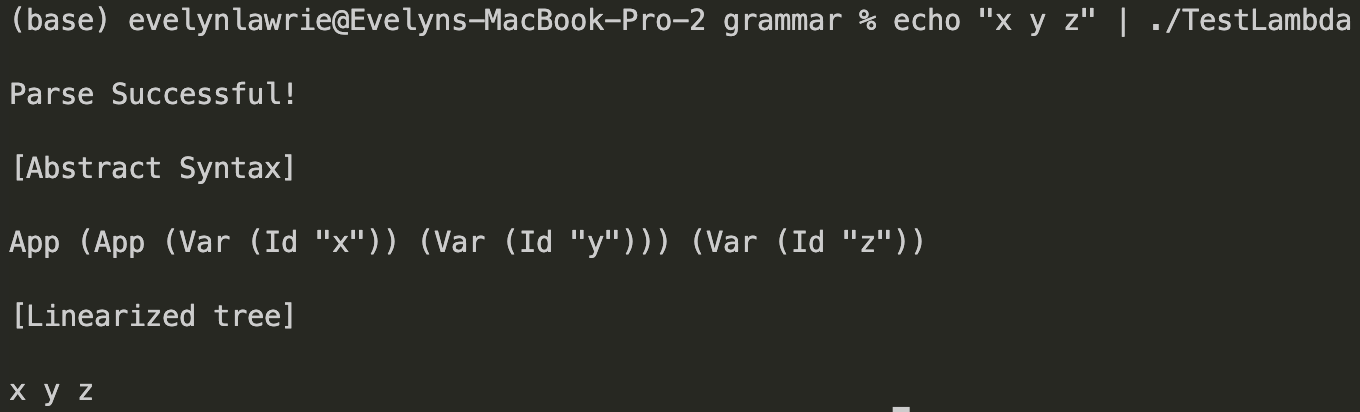
\includegraphics[scale=0.4]{img/ASTd.png}
\end{center}
\caption{x y z}\label{ASTd}
\end{figure}

\begin{figure}[H]
\begin{center}
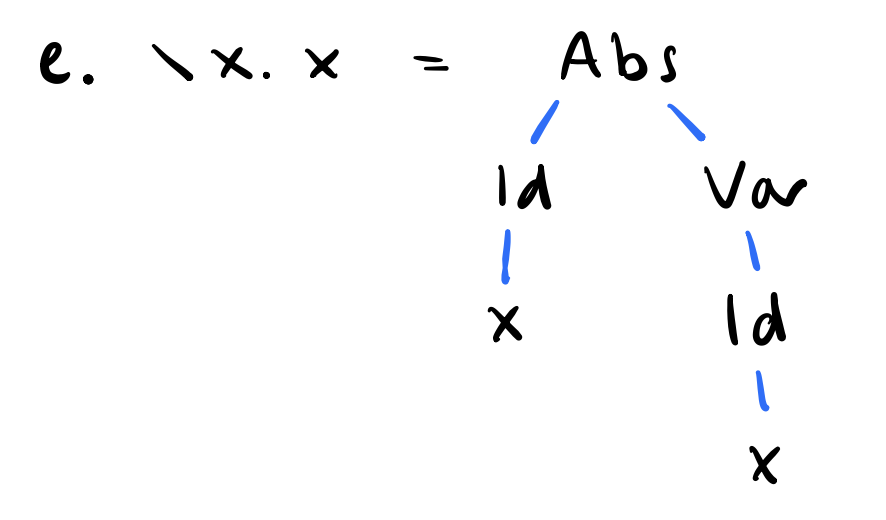
\includegraphics[scale=0.4]{img/eAST.png}
\\
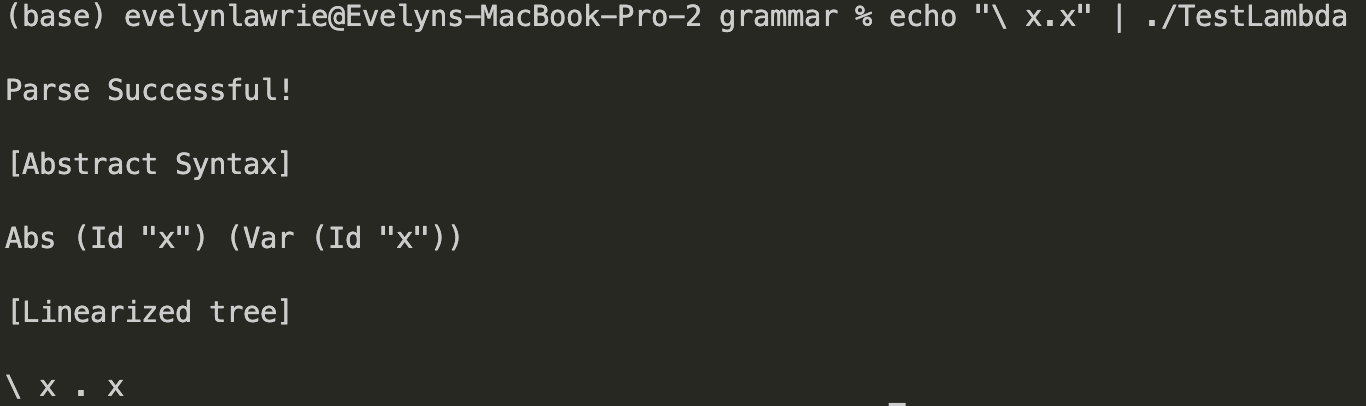
\includegraphics[scale=0.4]{img/ASTe.png}
\end{center}
\caption{$\lambda x. x$}\label{ASTe}
\end{figure}

\begin{figure}[H]
\begin{center}
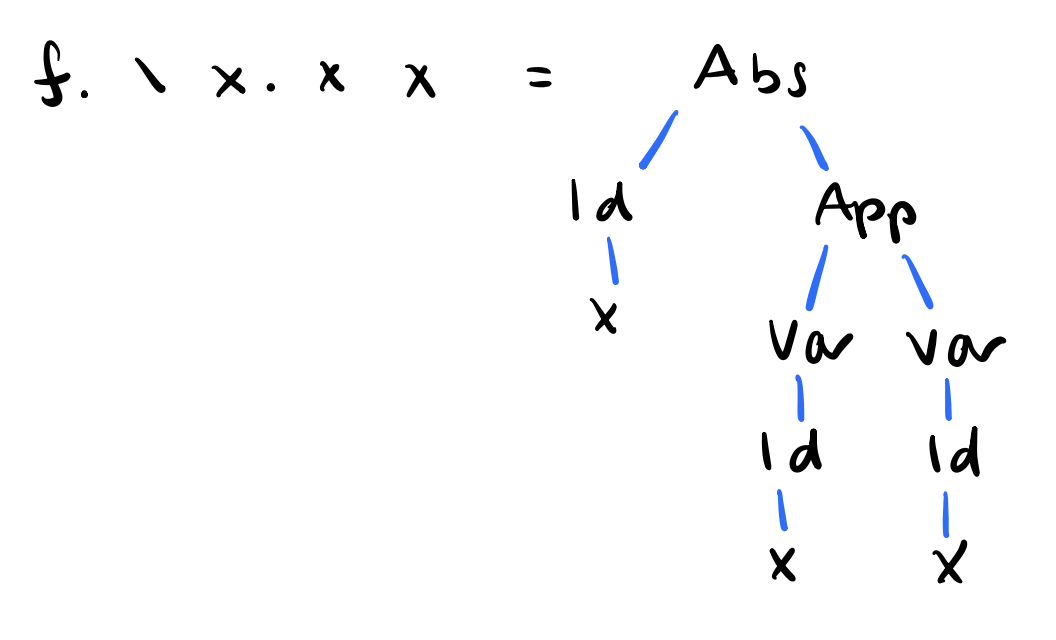
\includegraphics[scale=0.4]{img/fAST.png}
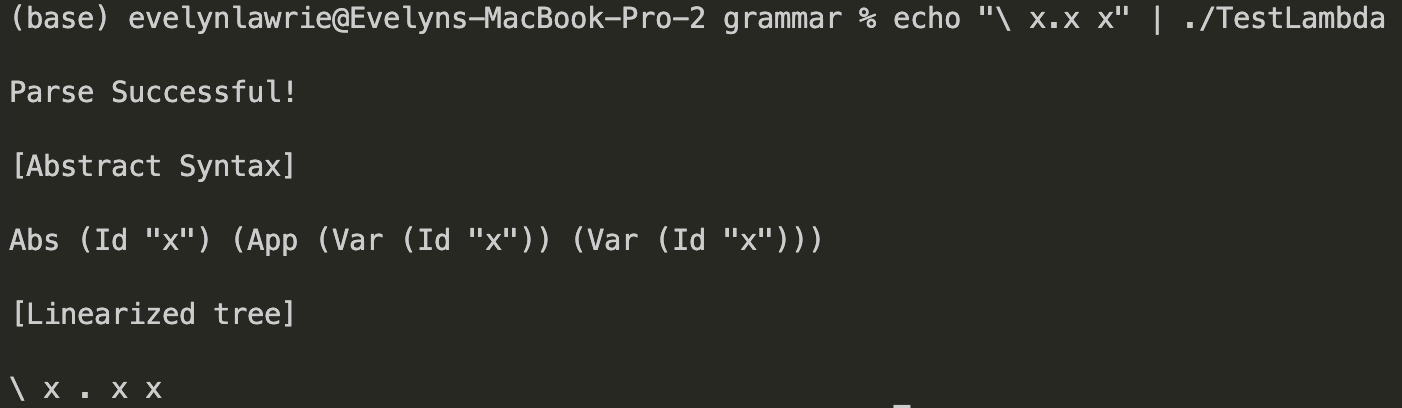
\includegraphics[scale=0.4]{img/ASTf.png}
\end{center}
\caption{$\lambda x. x x$}\label{ASTf}
\end{figure}

\begin{figure}[H]
\begin{center}
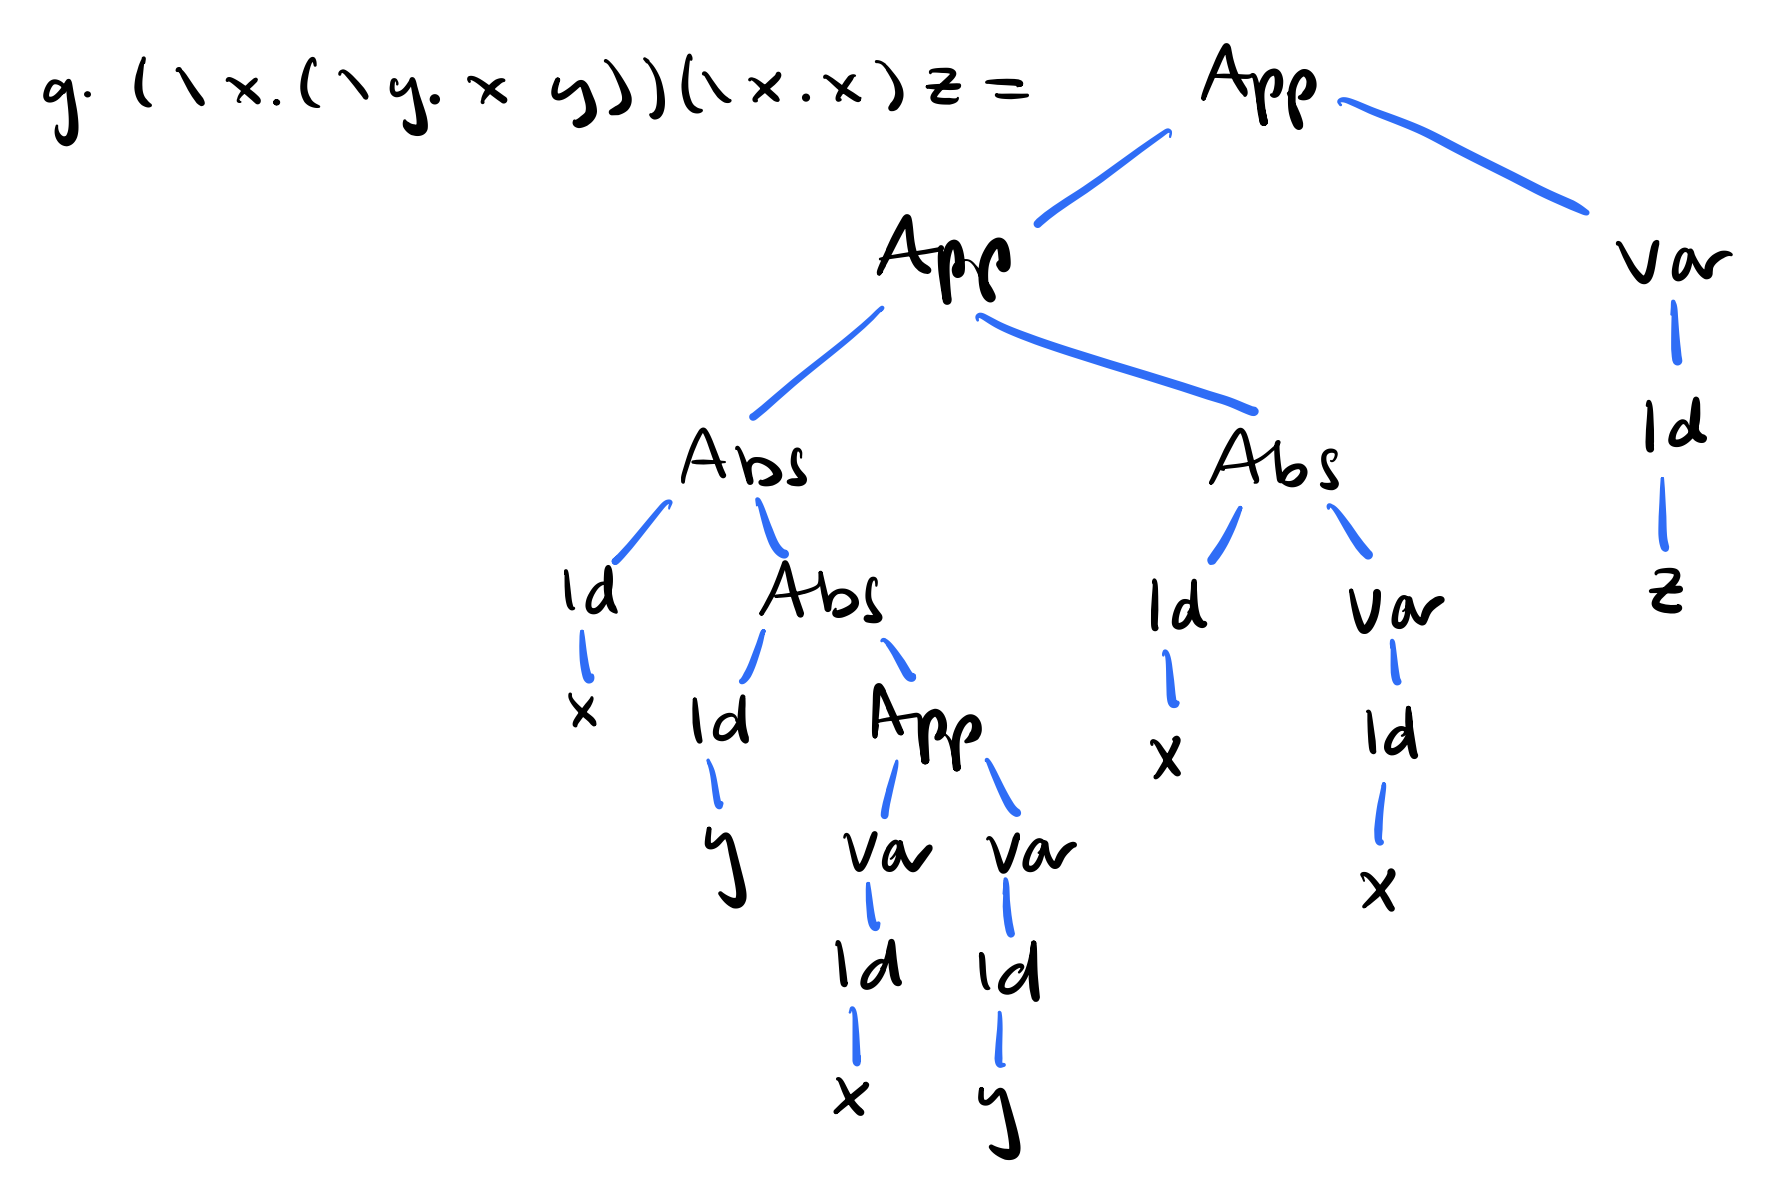
\includegraphics[scale=0.4]{img/gAST.png}
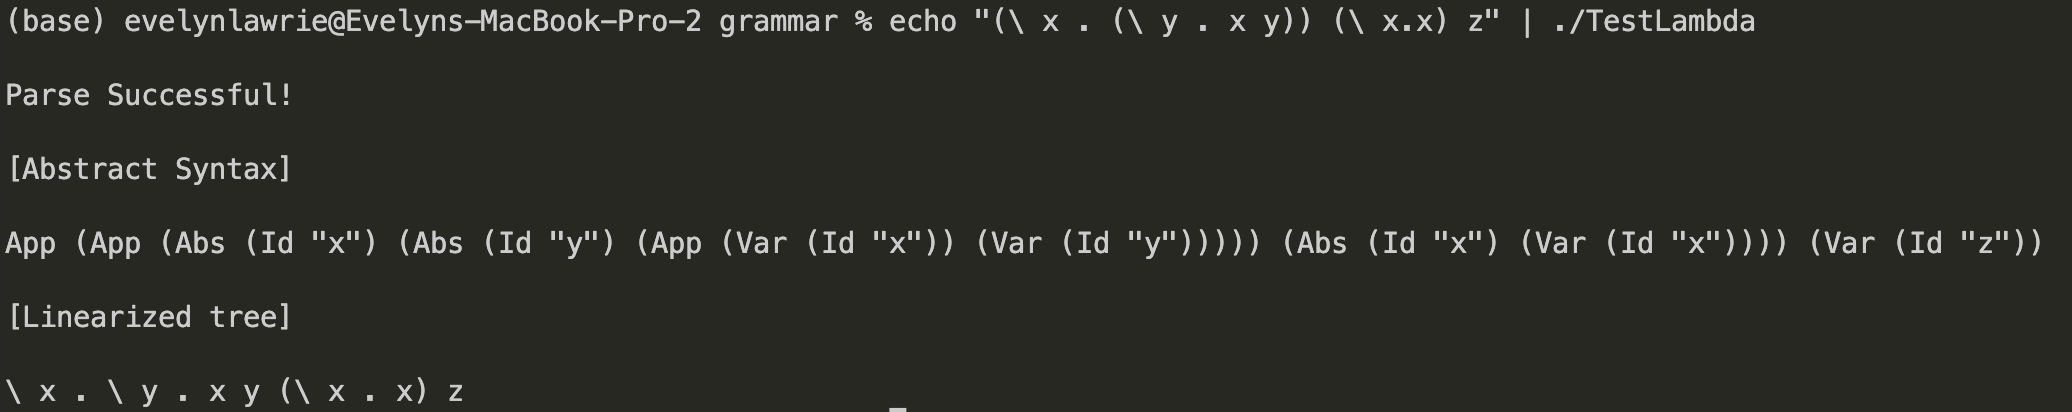
\includegraphics[scale=0.4]{img/ASTg.png}
\end{center}
\caption{$(\lambda x. (\lambda y. x y)) (\lambda x. x) z$}\label{ASTg}
\end{figure}

\begin{figure}[H]
\begin{center}
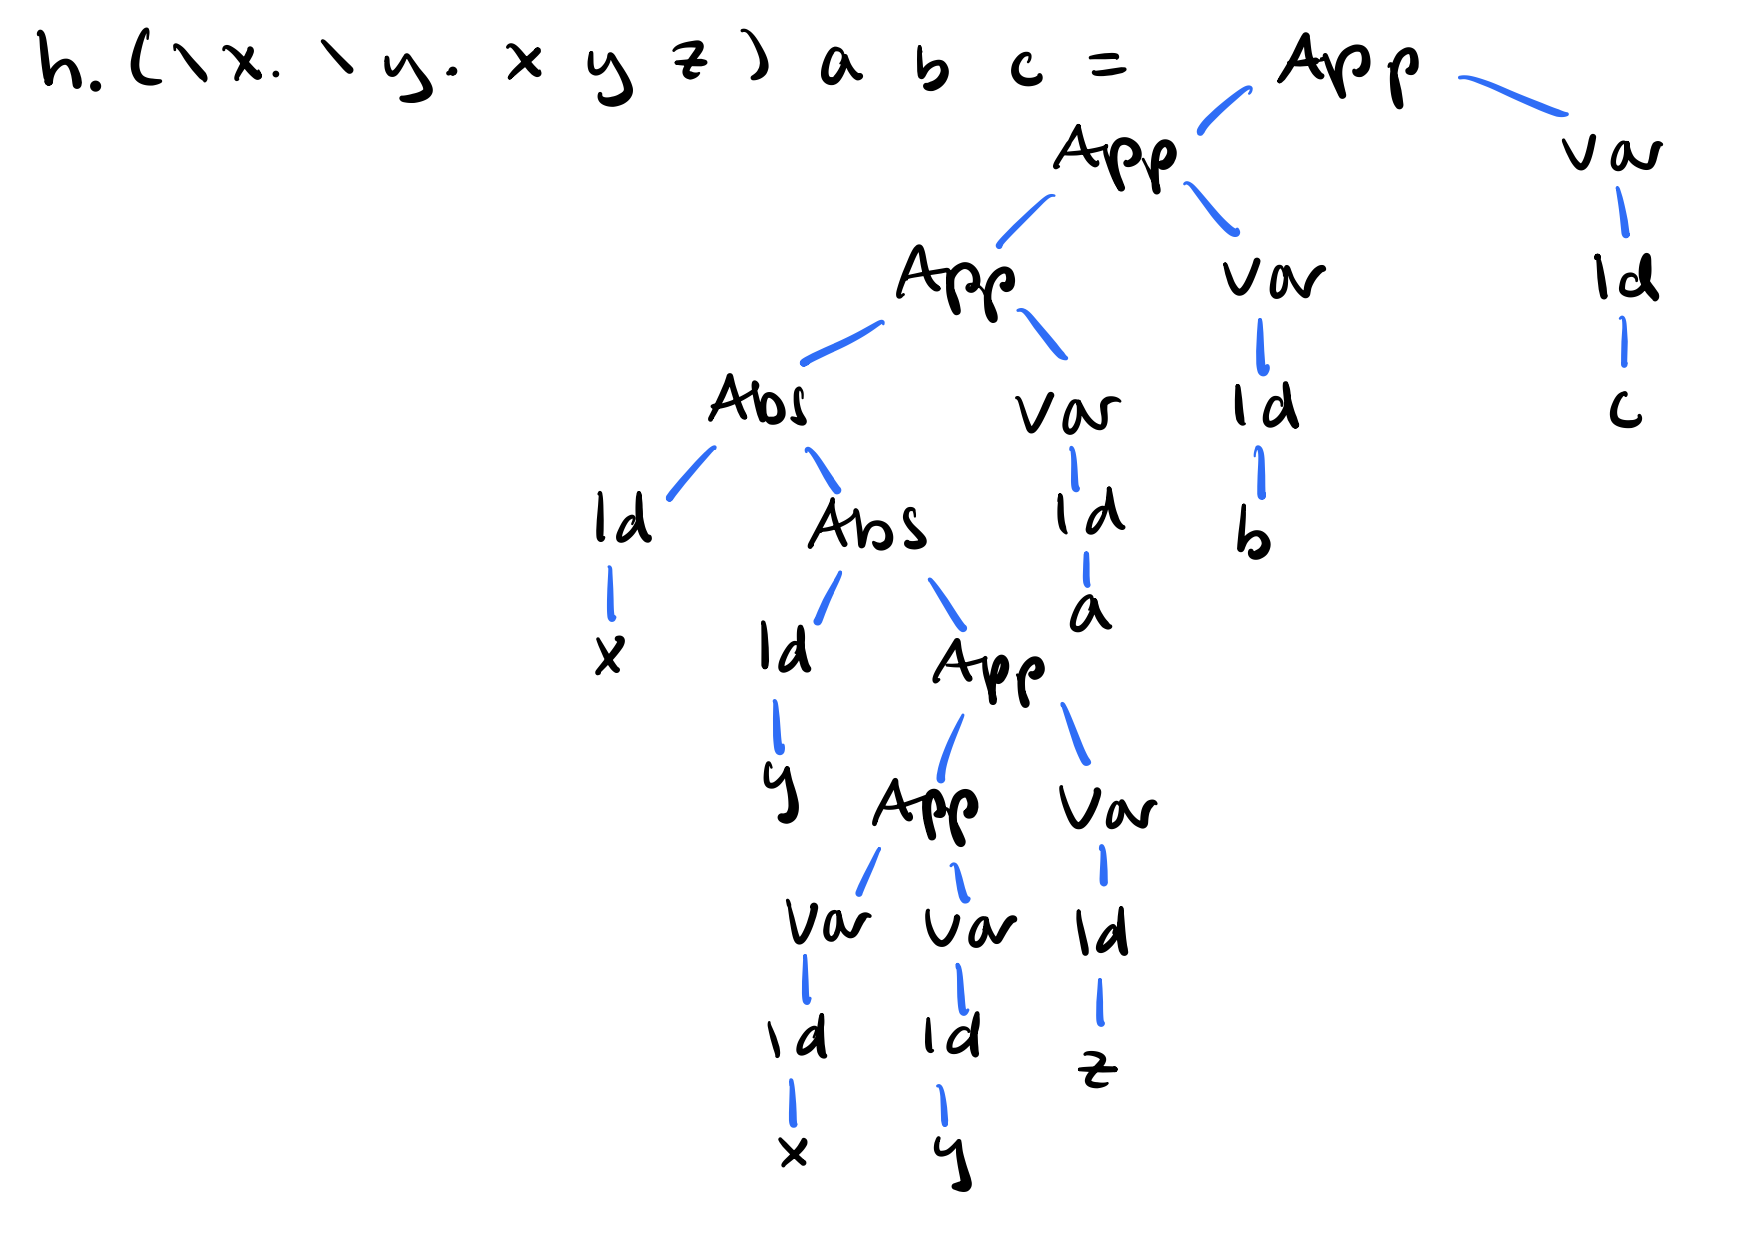
\includegraphics[scale=0.4]{img/hAST.png}
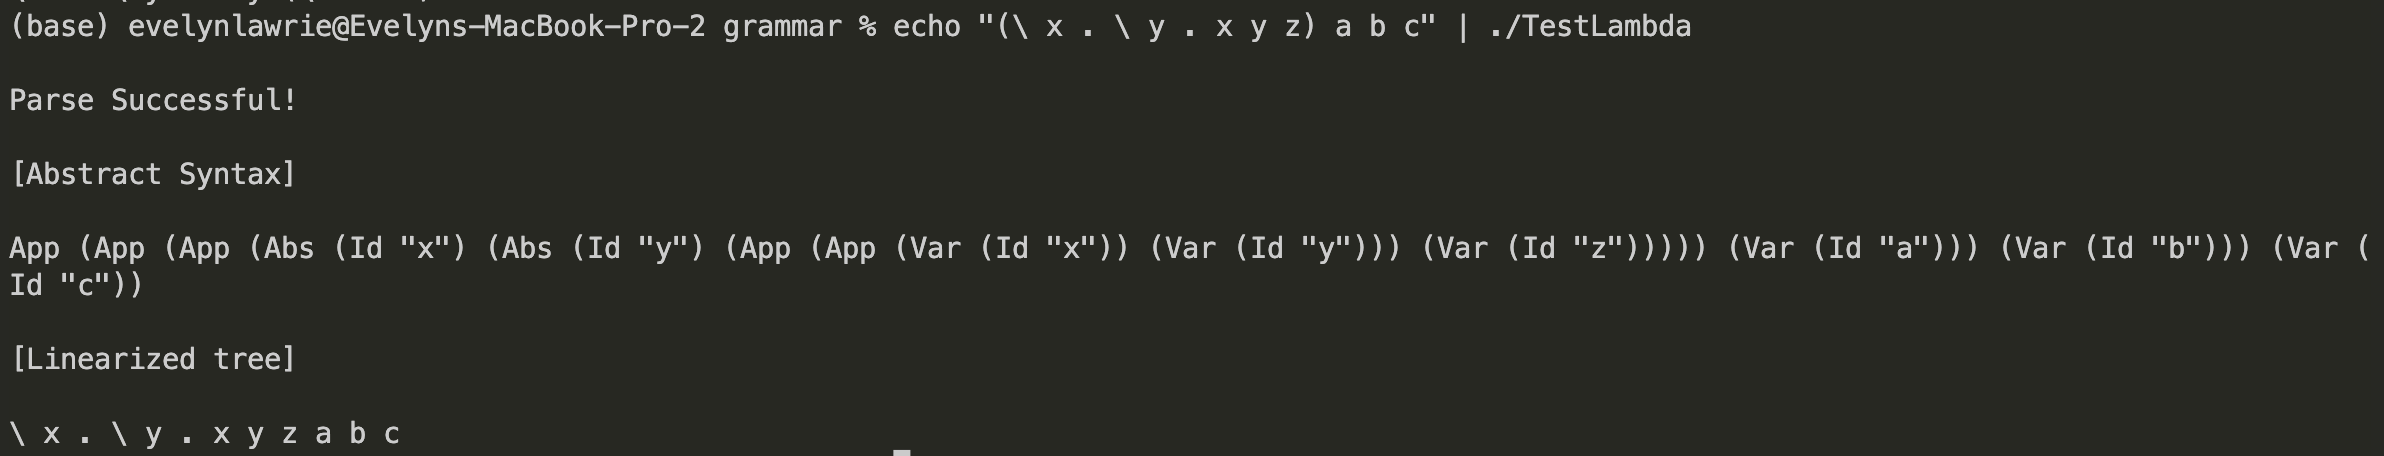
\includegraphics[scale=0.4]{img/ASTh.png}
\end{center}
\caption{$(\lambda x. \lambda y. x y z) a b c$}\label{ASTh}
\end{figure}

\subsection{Semantics}

The Lambda calculus semantics homework entails finishing the workout that we started in class. Below is an image of my typed out computation: 

\begin{figure}[H]
\begin{center}
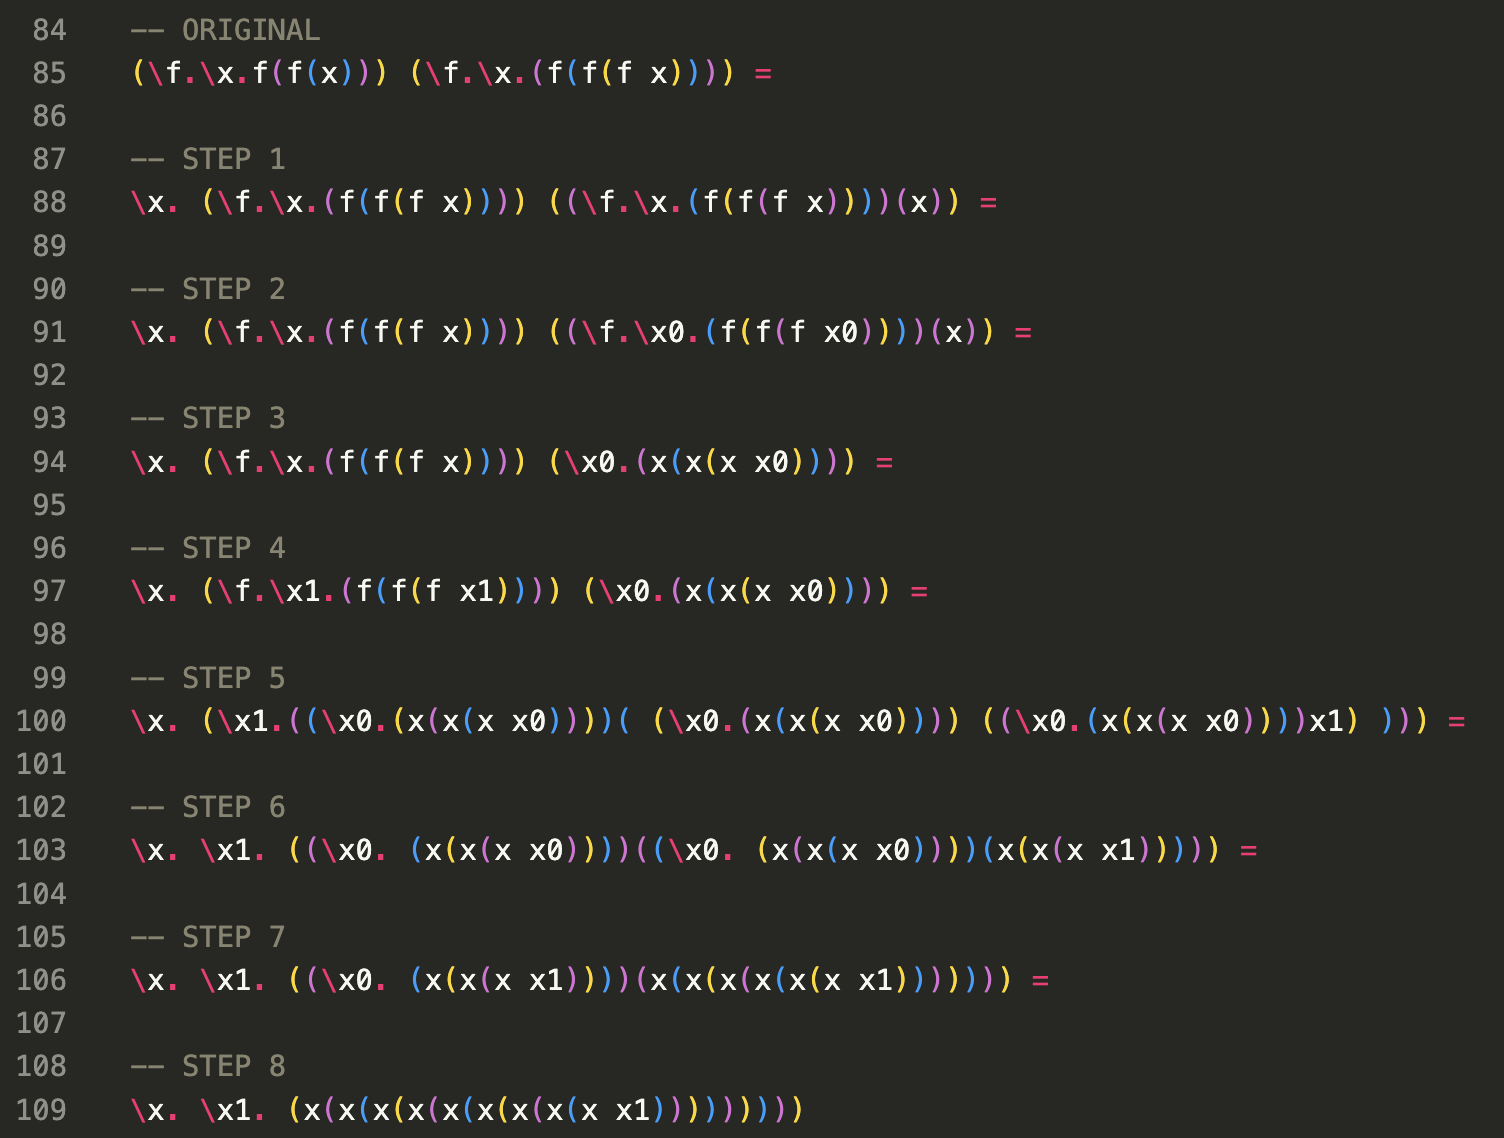
\includegraphics[scale=0.6]{img/workoutSolution.png}
\end{center}
\caption{Workout Solution}\label{WS}
\end{figure}

\subsection{Lambda Calculus Conclusion}

Week 4 gives us an introduction to Lambda calculus and its applications. Lambda calculus is the simplest possible programming language. The syntax may look very different to most programming languages, but it contains all of the same concepts. This allows us to strip back a lot of the syntax and get to the root of the basis of programming languages. To be able to write programs using only variables, abstraction, and application is a good starting point to understand the logic of why computer programs work the way that they do. Using variable binding and substitution for Lambda calculus computations (using the Alpha and Beta rules) teaches us how to rename formal parameters and perform capture avoiding substitution, which are the building blocks of Lambda calculus. In capture avoiding substitution, we rename the formal parameters (bound variables) and then replace that parameter in the body of the function by the argument. Reducing Lambda calculus expressions according to these rules demonstrates how this logic is computed by the machine in its simplification. We are able to better understand how computers interpret code by working step-by-step through these computations and having a foundational understanding of Lambda calculus as a whole. 

\section{Week 5}

\subsection{Introduction}

Substitution with function composition is discussed in this lesson, as the topics of free and bound variables come up when trying to implement function composition for functions that share variable names.

\subsection{Variables, Binding, Scope, and Substitution} 

Below is the correct formula for $f \circ g$ with $f(x)$ and $g(y)$ restated:

\begin{align}
f(x) = x + z \\
g(y) = 2 * y \\
f \circ g = f(g(y)) \\
= 2 * y + z
\end{align}

Because the variable $y$ in $f(x)$ is bound by $f$, it is a different variable than the one passed in by substituting $g(y)$ into $f$. To implement capture avoiding substitution, it is necessary to rename the variable $y$ in $f(x)$ to a different name (I chose $z$ in this case), making it a fresh variable. Therefore, this equation avoids ambiguity by separating variables that do not  hold the same meaning.

Below is a general formula for $f \circ g$ written in Lambda calculus:

\begin{align}
f \circ g = \lambda x. \text{ } f\text{ } (\lambda y. \text{ } g \text{ } y)
\end{align}

This formula works for any arbitrary functions $f$ and $g$ where the function $g$ gets applied to the argument $y$ in $g \text{ } y$ and becomes the argument for the function $f$. The result of $f \text{ } (\lambda y. \text{ } g \text{ } y)$ represents the composition of $f$ and $g$.

\subsection{Interpreting Lambda Calculus}

Using the file Interpreter.hs, below is the line by line evaluation of the expression $(\lambda x. \lambda y. x)y$:

\begin{lstlisting}
-- interpreter steps:
-- 1. evaluate original statement
eval (App (Abs (Id "x") (Abs (Id "y") (Var (Id "x")))) (Var (Id "y"))) 
--                (  i  )  (            e3              ) (     e2     )
-- 2. find App in eval function 
-- 3. apply line 10 
eval (subst (Id "x") eval (Var (Id "y")) (Abs (Id "y")(Var (Id "x"))))
--            (  i  )       (     e2     ) (           e3            )
-- 4. eval e2 just equals e2 since it's a variable 
-- 5. apply line 13  
eval (subst (Id "x") (Var (Id "y")) (Abs (Id "y")(Var (Id "x"))))
--            (  id  ) (      s     ) (Abs   id1         e1      )
--                                    (            e              )
-- 6. apply line 28 
-- line 29 
let f = fresh (Abs (Id "y")(Var (Id "x"))) 
--                   ( id1 ) (     e1    )
-- 7. compute fresh with the freshAux function
    -- compute line 21 
    fresh = Id . freshAux 
    -- find freshAux function that matches 
    -- apply line 19 
    freshAux (Abs (Id "y") (Var (Id "x"))) = ("y") ++ freshAux (Var (Id "x"))
--                  ( Id i ) (     e      )    ( i )             (      e      )
    -- evaluate freshAux (Var (Id "x")) 
    -- apply line 17 
    freshAux (Var (Id "x")) = "x" ++ "0"
--                     ( i )   ( i )
    -- f = Id "yx0"
-- line 30
    e2 = subst (Id "y") f (Var (Id "x"))
--               (  id1 )   (    e1/e    ) 
-- 8. evaluate e2 
    -- apply line 25 (this equation is true because id != id1)
    subst (Id "y") f (Var (Id "x")) = (Var (Id "x")) 
--          (  id ) (s) (   id1   )     (    id1    ) 
    -- e2 = (Var (Id "x")) 
-- line 31 
-- 9. compute this line 
    Abs (Id "yx0") (subst (Id "x") (Var (Id "y")) (Var (Id "x")))
--                            (  id  ) (      s     ) (     e2      )
    -- compute subsitution --> apply line 25 (this equation is true because id = id1)
    subst (Id "x") (Var (Id "y")) (Var (Id "x")) = (Var (Id "y"))
--          (  id  ) (      s     ) (     id1    )   (      s     )
    -- evaluate with line 12 
    Abs (Id "yx0") (Var (Id "y")) 
    eval Abs (Id "yx0") (Var (Id "y")) = Abs (Id "yx0") (eval (Var (Id "y")))
--             (   i    ) (      e     )       (   i    )       (      e     ) 
    -- evaluate eval (e) with line 13 (this equation is true because variables evaluate to themselves)
    eval ((Var (Id "y"))) = (Var (Id "y"))
--         (       x      )   (     x      )
-- final output of the evaluation = \yx0. y = 
Abs (Id "yx0") (Var (Id "y")) 
\end{lstlisting}

As for the binders and scope, for Lambda calculus substitutions that follow the form $(\lambda id.e)s$, this equation gets simplified in the code to $subst \text{ } id \text{ } s \text{ } e$. Therefore, for all calculations, $\lambda id$ is the binder and the scope of the binder is $e$. The scope of $s$ and the scope of $\lambda id$ are both $e$. The assignments of scope and binder are based on the pattern matching performed above, where each term assigned to $\lambda id$ and $e$ are the equivalents in each specific function call of $subst$. Below are the solutions for the binders and scope of the specific variables for each call to the function $subst$ in the above calculation: 

\begin{lstlisting}
-- Step 5 subst calculation:
subst (Id "x") (Var (Id "y")) (Abs (Id "y")(Var (Id "x"))) 
-- binder = (Id "x"), scope of binder (bound variable) = (Abs (Id "y")(Var (Id "x"))), free variable = (Var (Id "y")) 

-- Step 7 line 30 subst calculation:
subst (Id "y") f (Var (Id "x")) 
-- binder = (Id "y"), scope of binder (bound variable) = (Var (Id "x")), free variable = f

-- Step 9 subst calculation:
subst (Id "x") (Var (Id "y")) (Var (Id "x"))
-- binder = (Id "x"), scope of binder (bound variable) = (Var (Id "x")), free variable = (Var (Id "y"))
\end{lstlisting}

\subsection{Conclusion}

The takeaways from Week 5 surround the topics of capture avoiding substitution, pattern matching, and implementing Lambda calculus in Haskell code. Capture avoiding substitution contains lessons of free and bound variables. These topics are pertinent in programming, when topics such as static variables and variable scopes becomes important when dealing with overlapping variable names and ambiguous variable updates. In section 6.1, the formula for function composition deals with the scope of variables and the need to rename variables to perform capture avoiding substitution. Some definitions of different types of variables are as follows. A bound variable is one that can be renamed by a fresh variable without resulting in any changes in its meaning. A fresh variable is defined simply as one that has not been used before. Lastly, a free variable is a variable that is not bound by any particular binder. Dealing with the topic of capture avoiding substitution allows us to better understand the meaning and values stored in our variables when we program. It reminds us to create unique variables names and work towards avoiding ambiguity in overlapping namespaces. 

The Lambda calculus interpreter section of Week 5's homework details how the interpreter processes Lambda calculus computations implemented in Haskell. Working step by step through the given exercise taught us not only about Haskell syntax in more detail, but also how computers interpret code. We can better understand the interpretation step of computer program execution knowing how an expression gets decoded and which lines get evaluated. The exercise dealt with pattern matching to decipher what lines get executed when the given expression is evaluated by the interpreter. This is a logical exercise that strengthens our capacity to make sense of which lines of code are visited for any given expression. This can help with error prevention and debugging, as understanding the logic behind what the interpreter executes in a program can allow us to see any potential logic or syntax errors present more easily. 

\section{Week 6}

\subsection{Introduction}

Week 6 introduces the topic of ARSs (Abstract Rewriting Systems) and string rewriting. An ARS is made up of a language (a set of words) $A$ and rules $R$ for rewriting strings created withing the language $A$. An ARS is confluent if every branch-off computation (where there can be multiple rules applied to the same string) result in the same computation in a further step. This is to say, every peak of the graph of the ARS evaluation has a valley. An ARS is terminating if it does not consist of infinite computations. Finally, an ARS has unique normal forms if all elements have a unique normal form. This is to say, it is convergent, which means it is confluent and terminating \cite{Ars}. For an ARS to have unique normal forms, it must be confluent and normalizing, that is, every object in the ARS must have at least one normal form \cite{Ars}. 

\subsection{Rewriting: Introduction}

Below are a list of seven examples ARSs with pictures:

\begin{figure}[H]
\begin{center}
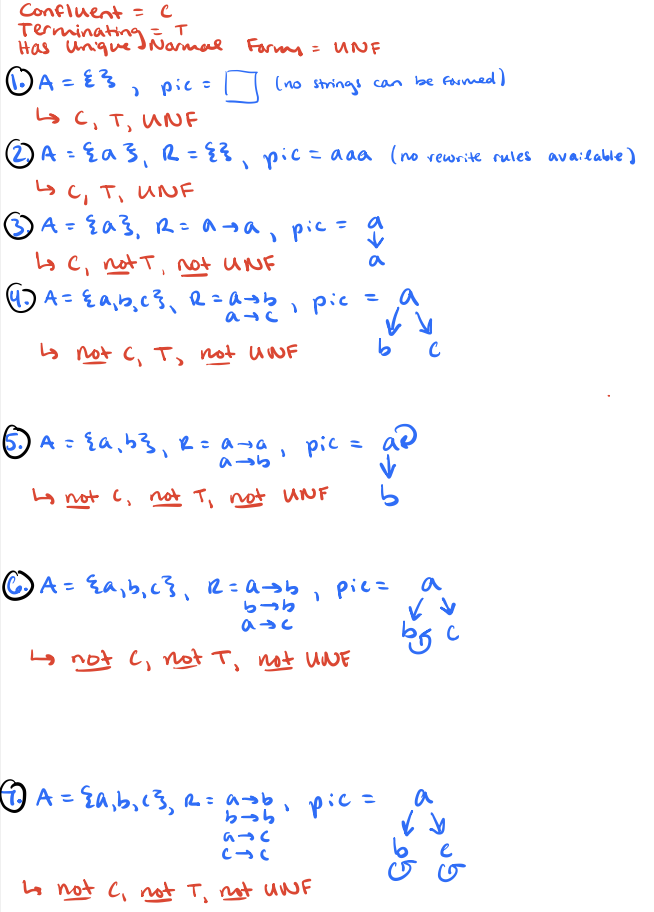
\includegraphics[scale=1]{img/ExampleARSs.png}
\end{center}
\caption{Example ARSs}\label{WS}
\end{figure}

Below is the table of examples of the 8 possible combinations of ARSs with pictures:

\begin{figure}[H]
\begin{center}
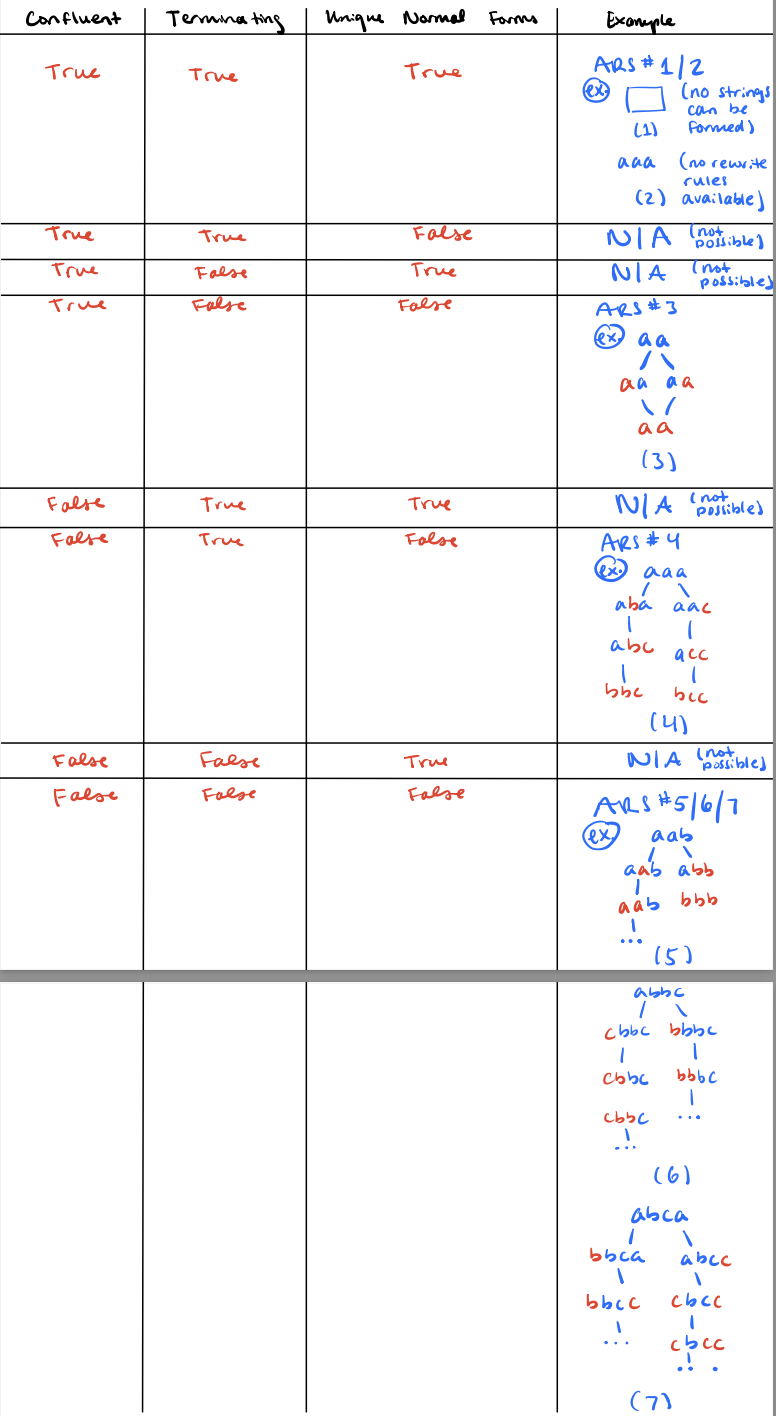
\includegraphics[scale=0.9]{img/ARSTable.png}
\end{center}
\caption{ARS Table}\label{WS}
\end{figure}

\subsection{String Rewriting Exercises}

This section explores further information on the topic of string rewriting. Below are the answers for the example computation, finishing the work we began in class:

\begin{lstlisting}
    aa -> a
    bb -> a
    ab -> b
    ba -> b
\end{lstlisting}

\noindent1. Why does the ARS terminate?
\\\indent This ARS terminates because it always reduces. There are no cases in which this ARS results in an infinite computation. This ARS is set up to get reduced to either the letter $a$ or $b$. 
\\
\\
2. What are the normal forms?
\\\indent The normal forms are $a$ and $b$.
\\
\\
3. Is there a string s that reduces to both $a$ and $b$?
\\\indent No, there are no strings in the ARS that evaluate to both $a$ and $b$ because the rewrite rules do not permit it. This is because the ARS is confluent: any combination of $a$ and $b$ evaluates to either $a$ or $b$; each string has unique normal forms.
\\
\\
4. Show that the ARS is confluent:
\\\indent This ARS is confluent because every peak in the reduction of a given string in the ARS has a valley that makes every branch in the computation reduce to the same final step. Below is an example of an overlapping critical pair that shows confluence of this ARS: 
\begin{figure}[H]
\begin{center}
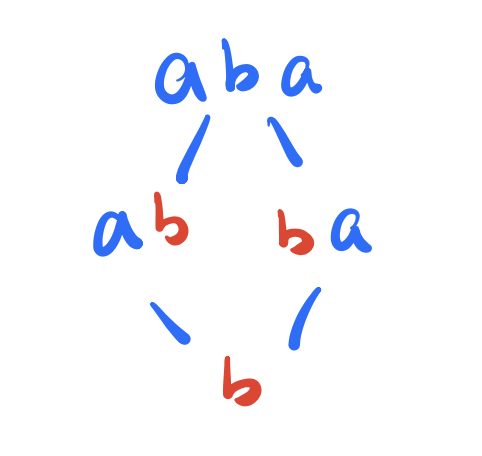
\includegraphics[scale=0.6]{img/ARSExample.png}
\end{center}
\caption{Demonstration of Confluence}\label{WS}
\end{figure}

\noindent5. Replacing $->$ by $=$,  which words become equal?
\\\indent Given the rewrite rules, $aa = bb$ and $ab = ba$. To generalize this statement, any word with an odd number of $b's$ = $b$ and any word with an even number of $b's$ = $a$.
\\
\\
6. What is the nicest way you can find to characterise which words are equal by one English sentence?
\\\indent Any words with an even number of $b's$ evaluates to $a$ and words with an odd number of $b's$ evaluates to $b$.
\\
\\
7. Repeat the last item using modular arithmetic:
\\\indent For any string $s$ in the ARS, $f$ is the frequency of $b's$ in $s$. $f \equiv 0 \text{ }(mod \text{ }2)$ shows if the frequency of $b's$ in $s$ is even or odd. Therefore, this formula written in modular arithmetic is as follows:
\begin{equation}
s = 
\left\{
    \begin{array}{lr}
        a, & \text{if } f \equiv 0 \text{ }(mod \text{ }2)\\
        b, & \text{otherwise}
    \end{array}
\right\}
\end{equation}
\\
\\
8. Which specification does the algorithm implement?
\\\indent This ARS represents an XOR logic gate, since the truth table of the rewrite rules outputs the same values as the logic for this gate. It determines whether there is an odd or even number of 1's ($b's$) in the original string. Below is an image of these truth tables to visualize their equivalence:

\begin{figure}[H]
\begin{center}
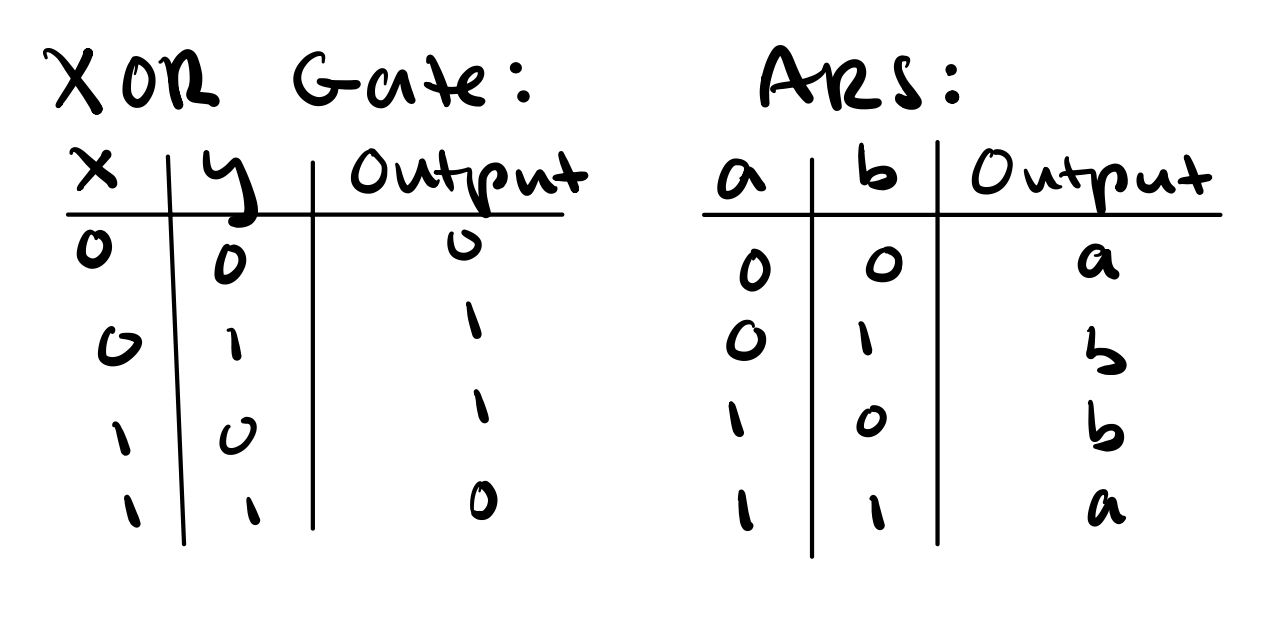
\includegraphics[scale=0.6]{img/TruthTable.png}
\end{center}
\caption{ARS and XOR Truth Table}\label{WS}
\end{figure}

\subsection{Rewriting Conclusion}

Week 6 taught us about Abstract Rewriting Systems. ARSs come with various classifications and elements. The topics of confluence, termination, and having unique normal forms were previously discussed. Evaluating ARSs for these qualities allows us to classify ARSs and better understand their behavior. Knowledge of ARSs can assist us in understanding Finite State Machines (FSMs) and automatons, since ARSs are simply unlabeled state transition systems \cite{Ars}. Since these are core topics in the fields of programming languages and algorithm analysis, they can assist with the comprehension of this field of computer science and logic. Here are a few other definitions that relate to ARSs that are key takeaways from this lesson and further our understanding of the topic:
\\\noindent 1. Equivalence:
\\\indent $a$ and $b$ are equivalente if $a \equiv b$, where $\equiv$ is the reflexive, symmetric, and transitive closure of the reduction arrow function $->$.
\\\noindent 2. Reduction:
\\\indent $a$ is reducible if if there is a $b$ such that $a -> b$.
\\\noindent 3. Normal Forms:
\\\indent $a$ is a normal form if $a$ is irreducible. Additionally, $b$ is a normal form of $a$ if $a$ reduces to $b$ and $b$ is a normal form. 
\\\noindent 4. Joinablity:
\\\indent $a$ and $b$ are joinable if they reduce to the same element.
\\\noindent 5. Local Confluence:
\\\indent For all $b$ and $c$ that are the outputs of two different rewrite rules in one given reduction step, the ARS is locally confluent if $b$ and $c$ are joinable. As well, if the ARS is terminating, local confluence implies confluence. 
\\\indent These definitions allow us to evaluate ARSs and the logic associated with them. Simplifying expressions of this type brings us back to topics such as reduction and simplification that we learned in high school algebra. Although this lesson implements these themes in a more structured way, we as students have been performing simplification in mathematics for years. These lessons strengthen our abilities to use logic and mathematical vocabulary, which we can apply to projects in our classes, future careers, and personal lives. 

\section{Week 7}

\subsection{Invariants Introduction}

In the realm of Abstract Reduction Systems (ARS), invariants play a pivotal role in unraveling the intricacies of system evolution. An invariant is a property that remains unchanged throughout the application of rewrite rules, providing a stable foundation for analysis and understanding. In the context of the given rewrite rules – transforming sequences of 'a's, 'b's, and 'c's – we delve into the exploration of invariants to discern patterns and constraints within the system's dynamic evolution.

\subsection{Option 2}

\begin{lstlisting}
Given the following rewrite rules:

    ab -> cc
    ac -> bb
    bc -> aa

and starting from 15 a's, 14 b's and 13 c's, is it possible to reach a configuration in which there are only a's or only b's or only c's?

Example calculations: 

    letters:                                   counts (parities):
    aaaaaaaaaaaaaaabbbbbbbbbbbbbbccccccccccccc 15,14,13
    accccccccccccccccccccccccccccccccccccccccc 1,0,41
    bbcccccccccccccccccccccccccccccccccccccccc 0,2,40
    baaccccccccccccccccccccccccccccccccccccccc 2,1,39
    ccaccccccccccccccccccccccccccccccccccccccc 1,0,41
    ccbbcccccccccccccccccccccccccccccccccccccc 0,2,40
    ...

    aabbcc 2,2,2
    accbcc 1,1,4
    bbcbcc 0,3,3
    baabcc 2,2,2
    ccabcc 1,1,4
    cbbbcc 0,3,3
    aaccbb 2,2,2
    ...

Invariant: 

    Two (or more) parities (counts) are always matching (even or odd) in each calculation step.
\end{lstlisting}

Based on the above calculations, reducing 15 a's, 14 b's, and 13 c's never allows for the possibility of reducing to a string with only a's, b's or c's. This is due to the invariant described above: two or more letters' parities are always either even or odd.

\subsection{Invariants Conclusion}

Week 7 dealt with invariants, which is a common topic in dealing with ARSs. We define invariants by thinking about what doesn't change in every step of an ARS's calculations. This is formally defined as: 
\begin{lstlisting}
P: A -> B is invariant of (A, ->) if P(A) = P(B) 
\end{lstlisting}
where change is defined as: 
\begin{lstlisting}
all a, b within A where a -> b.
\end{lstlisting}
This can allow us to better understand the behavior of ARS rewrite rules and further how to evaluate strings based on their criteria. Invariants help us find patterns in ARS  calculations that strengthen our logic processes. Invariants in hold a profound significance as they provide a stable foundation upon which to understand and analyze dynamic processes in various domains, from computer science to mathematics and beyond. These invariants are essential because they encapsulate characteristics that remain unchanged throughout an ARS's evolution. In a broader context, the study of invariants teaches us an important lesson about the fundamental principles governing change and transformation. By identifying and preserving these invariants, we gain insight into the underlying structures and symmetries that persist amidst complexity. This, in turn, deepens our understanding of not only ARSs but also real-world phenomena, enabling us to make predictions, ensure correctness, and design more efficient algorithms and systems. 

\section{Week 9}

\subsection{Peer Review Introduction}

This week's task was to evaluate another Blockly project. This gives us a feel for another implementation of the same project specification with a unique twist. Since the project that we were assigned is an application of a subtopic in machine learning, we approached our evaluation of this project through the lens of machine learning and its educational function in a block-based implementation.

\subsection{Conducting Peer Review}

The project my group was tasked to review is titled Energy Symbolic Regression. This project's objective is to apply the concept of symbolic regression using an energy-based approach, with a focus on modifying the loss function from the Hopfield neural network formula. In this review, I will be evaluating this project and the overall clarity of documentation provided. In peer reviewing this project, my group and I aim to provide insights and recommendations to enhance the project's quality and usefulness, particularly within the context of an educational environment. 

The project is centered around symbolic regression, a field in machine learning that seeks to discover mathematical expressions or symbolic representations that best fit a given dataset. An interesting novel element that this project introduces is the energy-based approach, replacing traditional data-centric regression methods with energy-centric ones. This has the potential to offer insights into alternative modeling techniques and further expand the toolkit for data analysis and modeling.

A few positive aspects of this project include the aforementioned use of energy-based symbolic regression is a novel concept that can potentially offer fresh perspectives on traditional regression problems. Another interesting part of this project is the incorporation of neural networks. The project demonstrates a clear attempt to integrate neural network concepts into symbolic regression, which is in line with contemporary trends in machine learning.

Below are a few areas of improvement for this project. There is a need for a clearer demonstration of how this project relates to the class's concepts. Providing a practical use case or illustrating how this approach can address real-world problems would greatly enhance the project's relevance. Since this project lacks a clear DSL (or any use of Blockly), it is difficult to determine how it fits in with the project specifications and our class's topics as a whole. There is also a clear lack of clarity in the documentation, especially for readers without a background in regression, neural networks, or machine learning. A step-by-step explanation of the project's components and how they interact would be immensely helpful. Clear explanations, along with code comments, would improve the project's readability and accessibility.

There is also an absence of information on running the project. Including a basic outline of the project's goals and clear instructions on how to interact with it would make it more user-friendly and beneficial to the intended audience. Lastly, the code lacks of comments and readability. Incorporating comments and structuring the code for better understanding is crucial for peer reviewers and users to grasp the project's intricacies.

The Energy Symbolic Regression project presents a novel approach to symbolic regression using energy-based methods. However, it requires significant improvements in documentation clarity, use case demonstration, and user-friendliness. Addressing these concerns will not only enhance the project's educational value but also make it accessible to a broader audience. With these enhancements, the project has the potential to be a valuable addition to the field of machine learning and symbolic regression.

As for my feedback on the peer review process as a whole, I found that in this format it does not yield the expected benefits or contribute substantially to the quality of the work of our projects. This is because we already had opportunities to give feedback on other projects in previous discussion posts, and having the projects assigned to us to review creates more confusion when the projects don't exactly line up with domain expertise. I see that there is a correlation between each of the groups' topics and I understand that every project needs reviewing, and it is good practice to work with GitHub issues and pull requests. I just personally feel that the peer review process could have been structured in a way that was more beneficial to us. It would have been better if we could have had one week to solely explore a repository, raise issues, and correct our issues. Then, another week could have been making the pull request and adding functionality. Having just one week to perform all of these tasks did not give any time for the other group to fix our issues before the deadline to submit a pull request. Also, it was difficult getting assigned a project that did not use Blockly, as the learning curve hindered our ability to thoughtfully contribute to the project. Overall, I believe that it would have been more beneficial for us to have used these weeks to continue adding functionality to build out the implementation of our project, since we have had previous peer review opportunities in this class and it felt as though we did not have ample time to make significant improvements to each other's projects. 

\subsection{Peer Review Conclusion}

Our review of the Energy Symbolic Regression project details our proposed areas of improvement, such as clearer documentation, code, and organization of the project. We believe that our recommendations would make this project more accessible and improve its ease-of-use. Since this project is not based in Blockly, we had some difficulty in understanding and implementing a pull request for our evaluation of this project. This review offers a thorough review that points out the areas of success and growth of the Energy Symbolic Regression project. 

\section{Week 10}

\subsection{Prisoner's Dilemma Introduction}

In the topics of coding and game theory, the Blockly Prisoner's Dilemma project emerges as a unique intersection, blending the strategic elements of decision-making with a technical programming implementation. This assignment delves into the inner workings of the project, employing the versatile debugger in VSCode to guide us through the complexities of the code.

\subsection{Blockly Prisoner's Dilemma}

1. Use the debugger to step through the code and explain what happens? \\

Initially, both participants must undergo registration to ensure the proper functioning of the game, with both individuals operating within the same port. Following this, they configure their block codes, ideally featuring an initial move (possibly a second move) and subsequent moves that may be contingent on the preceding ones. Alternatively, the moves can consistently be either defect or cooperate. Subsequently, once both players' codes update the program's value dictionary, it progresses through five rounds, evaluating who defected and who cooperated based on the specified logic. Additionally, a one-second interval timer continuously prints on the console until the second player makes their move. \\

\noindent2. Under which conditions do both players get the result of the game? \\

Both players receive the game result when both employ strategies such as always defect or always cooperate. However, when conditionals are present, and a player's move depends on the other player's last move, a conclusive output may not always be obtained.\\

\noindent3. Why can it happen that only the second player gets the result?\\

This occurs when the first player has executed their move, but the second player has not yet made their move. Consequently, only the second player receives the result, as the computation takes both players' moves into account.\\

\noindent4. What would be a way to improve on this?\\

An improvement could be achieved by notifying one player that the other has made a move. Alternatively, a message could be sent indicating that a player has exited the game. This would provide clarity, ensuring that the participant is aware of the other player's involvement rather than leaving them uncertain about being the first to make a move or questioning whether the other person has exited.\\

\noindent5. Describe how you used the debugger and what you learned from it:\\

I employed the debugger to inspect the backend processes via terminal input, enabling me to confirm the information exchanged between players. Witnessing the modularity and logic of the program operating in the back-end provided valuable lessons. Learning how to use a debugger is applicable for software development and future coding projects we implement. 

\subsection{Prisoner's Dilemma Conclusion}

Week 10 dealt with using a debugger in VSCode to evaluate the Blockly Prisoner's Dilemma project. Typically, the Prisoner's Dilemma project is introduced solely from an economic or political science perspective, but delving into its technical aspects revealed a different layer of understanding. Getting to see how this problem works behind the scenes teaches us about a complex situation and how to evaluate it using code. Especially implementing it using Blockly gives us a beginner friendly functionality to teach us as well as any potential users about the logic of this problem. This was also the first time I had used a debugger, which is a useful tool in VSCode. Getting to see how this program works behind the scenes and line-by-line how the computer executes it gives us useful insights on how this program works. We can apply this debugger tool to our future projects as it can help us diagnose issues more systematically and approach debugging in a detail-oriented way.

\section{Lessons from the Project}

Throughout the semester, this Blockly project tested our communication and collaboration skills. My group consisted of four members, and making sure we scheduled meeting times where we were all present to work together was a challenge. Thankfully, we all prioritized open communication and made sure that our work was split evenly each week. We followed an Agile Scrum methodology, as this was what the incremental project deadlines allowed for. We developed our project according to the given guidelines and made sure we were pivoting and maintaining adaptability when possible. This allowed us to be successful in this project, as we were able to make alterations to our project when guidelines would change. This also allowed us to learn from feedback given to us, as we were able to collaborate to bring suggestions on board that we received during our midterm presentation. For example, some feedback we received brought up the fact that more documentation provided on our Blockly interface would be helpful to guide users through the page and allow them to understand what the blocks mean. Specifically, for setting up the variables for training and targets, it is imperative to know what the features of the dataset are in order to know what variables are available to use. To that end, we added a documentation section to our interface with blocks that provide links for users to explore the datasets as well as get more information on the other elements of our project. This allows them to go beyond our Blockly interface and learn the behind the scenes of why these blocks work the way they do to provide a basic machine learning pipeline. 

As for the tools we used, Git and Visual Studio Code proved key in our software development process. We got experience working with different branches in Git and resolving merge conflicts. Because there were only a few files to work on throughout this project, it was at times difficult to split up the work and have multiple students working on the same file at once due to potential merge conflicts. So we implemented lots of pair programming and collaborated on one laptop to avoid those conflicts at times. This aided our debugging process, as multiple of us were able to look through the code at once. Working via different branches also helped with this issue. Another tool we were required to use was GitHub Pages for displaying our Blockly project interface. This proved difficult when our Pages would not update when we made changes or source the index.html file from the correct directory. We had many issues when tasked with creating different versions of our project for peer review or midterm progress reports. This changed up the file that the pages was getting its information from and it was difficult to figure out how to resolve these issues. One element of feedback I would have is to eliminate Github pages from the project requirements. It is a useful tool, but it provided many issues for us and other groups that it seemed like more trouble than it was worth. In future implementations of the Blockly project, it would be extremely helpful if we could go over how to create a GitHub pages site in class because it felt like we were thrown in the deep end with its implementation and unaware of the exact guidelines for what the site should look like and where it should be sourcing from. 

This project provided us with useful skills in JavaScript and HTML development. This is a useful application for our careers as software engineers, as web development is a critical skill and involves in-depth knowledge of these tools (JavaScript especially). Getting to use built-in libraries and functionality with the Blockly toolkit is applicable as well, since a lot of web development (and programming in general) consists upon pre-defined frameworks to improve projects stylistically and build upon their functionality. Knowing how to manipulate these toolkits is critical. In our case, this entailed defining custom blocks for the unique functions of our program. We were able to explore documentation and other examples of Blockly projects to understand exactly how to customize the Blockly functionality to work for what we wanted our implementation to be. Blockly in itself is a useful learning tool as it is a block-based program that gives users an introduction to any certain topic. Block-based programs are useful as a basis for learning programming for the first time, as tools like Blockly and Scratch are widely used to give an introduction to the various components of programming before concerning users with syntax. In this sense, using Blockly to create our own DSL applied the topics of programming language creation to a simplified interface to allow ease of use and interaction with the platform. 

Since our project provided an educational tool for an introduction to machine learning, our group gained lots of experience and knowledge on this topic throughout the semester. Our project detailed a machine learning pipeline that provided code for users to test and manipulate. This meant that we had to provide the code that was generated by these blocks, which meant gaining an in-depth understanding of the different steps to take to implement a machine learning model and its evaluation. We provided blocks for some data visualizations that provide exploratory data analysis functionality to get the users more familiar with the given dataset. We also implemented model selection, training, and evaluation blocks to give users a basic workflow to perform analysis using on of the six models that we provide users to choose from. We determined these models based on their varying complexities. We provide users with more basic as well as more nuanced models to give them a basic introduction to machine learning models while also providing them with the opportunity to explore more complex models and ones that build on each other. Machine learning is a very prevalent topic today, as the recent emergence of AI is making these technologies ubiquitous in our society. Machine learning and AI are closely intertwined fields, with machine learning serving as a key component of AI. Essentially, machine learning is a subset of AI that focuses on the development of algorithms and statistical models that enable computers to improve their performance on a specific task over time without being explicitly programmed. The relationship between machine learning and AI is symbiotic, as machine learning provides the tools and techniques that allow AI systems to learn from data and make intelligent decisions. Using our Blockly program as an introduction to machine learning provides a useful tool to users to gain an introduction into this topic that is so important today. It also provided all of us working on the project a more in-depth understanding of this field of computer science, given our varying prior experience with the topic. Even though we had varying levels of experience, all of us were able to equally contribute to the project and we all gained understanding of the subset of machine learning that we worked on implementing in the interface. This proved to be an effective method of project development, as we split up the work in a way that played to our strengths and allowed us to each make substantial contributions. 

Our code contained nine different subsections of blocks to separate our code into easily readable sections. Our first section, Datasets, contains the functionality for importing our built-in datasets or a custom dataset (by using a text input field on a custom dataset block). This allows for the utilization of any of these datasets within the program on which to perform data analysis and machine learning. We learned from this section how to read data through links into the Blockly code in JavaScript. The next section is Input Data, which deals with reading and printing the data imported with the blocks in the Datasets section. The Print CSV Data block allows the user to visualize the data and is meant to be run on its own and pasted in an individual cell in Google Colab. The Read CSV block allows for turning the dataset into a data structure that the program can understand to pull features from and evaluate, namely a Pandas dataframe. Next, the Data Visualizations section allows for creation of a scatterplot or bar chart. These visualizations allow the users to better understand how different variables in the model affect the target variable or value the user wants to predict. Through the various customization options, we allow users to create the graph of their choice and visualize how the different possible parameters interact with each other. This can allow users to be more informed when they select the variables they want to use to predict the categorical or continuous values. The next section allows for data cleaning, titled Clean Data. This section provides blocks to normalize the data, drop null values from the data inputted, and select certain attributes from the array for further analysis. The normalize data block uses the StandardScaler module from the sklean library. The StandardScaler is a preprocessing technique commonly used in machine learning to normalize or standardize the features of a dataset. Normalization is important when the features of a dataset have different scales, as it can help improve the performance and convergence of certain machine learning algorithms. The StandardScaler operates by transforming the data such that it has a mean of 0 and a standard deviation of 1. For each feature, it subtracts the mean value of that feature from each data point and then divides the result by the standard deviation. This process ensures that the features are centered around zero and have a consistent scale, making it easier for models to learn patterns without being biased by the inherent scale differences between features. StandardScaler is particularly useful when working with algorithms that rely on distance metrics, such as k-nearest neighbors or support vector machines. These models are among the ones that we offer to users to choose from for their analysis, so normalizing data is an imperative part of our machine learning pipeline. 

Moving into our model creation and analysis portion of the project, we have a block category called Model Training that takes in blocks from the Model Selection and Train/Test Split categories. The block that gets inputted into the Training Data section of the Model Training block is the data outputted from the Train Test Split block. This block performs a train/test split on the normalized data inputted into it. We allow users to select attributes from the dataset with the blocks in the Clean Data section, so that they can choose which features to use for the analysis. The train/test split block also allows them to select a target variable, the one that they want to either predict or classify. Train/test split is a fundamental concept in machine learning that involves dividing a dataset into two subsets: a training set and a testing set. The training set is used to train a machine learning model, while the testing set is used to evaluate the model's performance on unseen data. The primary goal is to assess how well the model generalizes to new, unseen examples. Typically, a random or stratified split is performed, allocating a certain percentage of the data to the training set and the remaining portion to the testing set. This separation helps prevent the model from memorizing the training data (overfitting) and allows for a more realistic assessment of its predictive capabilities. By evaluating a model on independent data, practitioners can gauge its performance and make informed decisions about its effectiveness, ensuring that the model is robust and applicable to new, unseen instances. The model selection blocks allow the users to choose either a classification or regression model based on the format of their target variable and what value they are trying to evaluate. Regression and classification are two main types of supervised machine learning models that serve different purposes. Regression models are used when the target variable is continuous, meaning it can take any numerical value within a given range. These models predict a quantity, such as predicting house prices, stock prices, or temperature. In contrast, classification models are applied when the target variable is categorical, meaning it falls into distinct classes or categories. Examples include spam detection, image recognition (identifying objects or faces), or sentiment analysis. The choice between regression and classification depends on the nature of the problem and the type of output variable you are trying to predict. If the goal is to predict a numerical value, regression is suitable; if the goal is to assign instances to predefined categories, classification is the appropriate choice.

The next category of blocks that we created were for model evaluation. We provide two different techniques for model analysis on both regression and classification models. For regression models, we provide the options to perform Mean Squared Error and R-squared analyses on the users' models. Mean Squared Error (MSE) and R-squared (R2) are both metrics used to evaluate the performance of regression models, but they capture different aspects of model accuracy. MSE measures the average squared difference between the predicted values and the actual values. It gives equal weight to all errors, penalizing larger errors more heavily. A lower MSE indicates better model performance. R-squared, on the other hand, represents the proportion of the variance in the dependent variable that is predictable from the independent variables. It ranges from 0 to 1, where 1 indicates a perfect fit. R2 provides an indication of how well the model explains the variability in the data. While both metrics are useful, the choice between them depends on the specific goals of the analysis. If the emphasis is on understanding the proportion of variance explained, R2 is valuable. If the focus is on the precision of individual predictions, MSE is more appropriate. It's common to use both metrics together to gain a comprehensive understanding of a regression model's performance. For classification models, we provided users with the choice to evaluate these models using Accuracy Score or a Confusion Matrix. Accuracy score and confusion matrix are two evaluation methods commonly used for assessing the performance of classification models. Accuracy score measures the overall correctness of predictions by calculating the ratio of correctly predicted instances to the total number of instances. While accuracy is intuitive and easy to interpret, it may not be suitable for imbalanced datasets, where one class significantly outnumbers the others. In such cases, accuracy may be high even if the model performs poorly on the minority class. On the other hand, a confusion matrix provides a more detailed breakdown of the model's performance by showing the number of true positives, true negatives, false positives, and false negatives. This information allows for the calculation of metrics like precision, recall, and F1 score, which can be more informative, especially in imbalanced scenarios. The choice between accuracy and a confusion matrix depends on the specific characteristics of the dataset and the importance of correctly identifying each class, guiding users to select the most relevant metric for their classification problem.

Our last category of blocks is titled Documentation. We provided a documentation section to our project to provide users with more information on each specific aspect of the machine learning pipeline. We hope the links we provided along with our block-based interface provide users with a beginner friendly introduction to machine learning.

In our educational tool BlocklyML, we aim to incorporate essential concepts from this class's lectures such as parsing, interpretation, and compilation. This integration provides users with a platform to practice machine learning principles through visual programming based on Blockly. Parsing, a key feature, allows users to input data in the form of CSV files. The tool then extracts and transforms this data into organized representations suitable for input into machine learning models, streamlining the data cleaning and transformation process.

Furthermore, our tool supports interpretation, aiding users in understanding their data. Through user-friendly Blockly-based visual programming, users can interpret data characteristics, relationships, and potential features, gaining deeper insights into their datasets. Visual representations of data pipelines, model architectures, and training processes enhance the comprehension of machine learning concepts.

Compilation principles come into play as users construct machine learning models using our tool. The visual blocks and connections crafted by users are translated into executable machine learning code, ensuring the accuracy and efficiency of the models. By seamlessly integrating parsing, interpretation, and compilation into our machine learning educational tool, we empower users not only to apply machine learning techniques but also to grasp the foundational processes of parsing, interpretation, and compilation using visual code blocks. This enhances their overall proficiency in data science and machine learning.

The project's interconnected blocks can be likened to the construction of an Abstract Syntax Tree, which was a key topic explored in this course. Users assemble these blocks to create models, illustrating how theoretical concepts can be practically implemented. This connection between the project and abstract syntax and implementation underscores the importance of modularity in BlocklyML. This alignment with theoretical principles, previously discussed in the context of programming languages, echoes back to earlier recursive concepts, as BlocklyML is constructed from smaller, reusable components. This adherence to modularity is a fundamental principle in recursion, as well as in the realms of programming languages and software engineering. BlocklyML's overall design philosophy delves into the exploration of functional programming concepts and their influence on language design. It emphasizes the use of clear, functional blocks that users can piece together to build intricate machine learning models.

Overall, this project taught us many lessons over the semester. We learned how to effectively collaborate and communicate, working as a team and playing to our strengths. We strengthened our knowledge on machine learning and the various subtopics within this branch of computer science. We also saw some of the course material come to life in this block-based implementation of a domain-specific language. We hope to have given users a platform to learn about machine learning in a way that is easy to navigate, understand, and customize. 

\section{Conclusion}\label{conclusions}

This report details various logical problems and their solutions implemented throughout this semester. As illustrated in this report, these algorithms can be approached in various different ways. Exploring different approaches to the same problem hones the skill set of novel solution creation, which allows programmers to complete tasks by thinking outside of the box in ways that seem less than straightforward. The thought processes behind the solutions to these problems can be applied to technical interviews, future computer science courses, and projects assigned in the workplace within the field of computer programming. The problem-solving techniques developed in this class and through this report serve as a basis of knowledge to assist students with our future endeavors. This is the way in which this course can fit into the wider world of software engineering, by developing our abilities to think outside of the box and develop novel solutions to complex problems. This skill will prepare us for ambiguous tasks that will be abundant in our careers as software engineers. 
 
The lessons that were most interesting to me were those in which we had to decipher and draw our abstract and concrete syntax trees. I found this section the most useful and engaging, as it was centered around logic and following the rules provided. I found this to be an intuitive exercise that was enjoyable to work through. This was a useful part of the homework since it taught us about how programs are executed, specifically how lambda calculus functions. It helped further my understanding of the App and Abs functions and how the computer evaluates them. 

As for improvements to this course, I would suggest that we worked through more practice problems in class to solidify our understanding of the course material. At times, I felt unprepared going into the homework as some weeks it presented us with an application of the material that we did not necessarily cover in class. I found myself unable to follow along with the course at times given its theoretical nature. Because of this, I think the material could have been presented in a simpler way since I know that a lot of us are not able to grasp such complex topics the first time around. And if in class it is clear that we are not able to follow along, it would be great if we could be presented with the information in multiple ways or using more concrete examples. If we had more time in class to work through examples in groups or as a class, this would have made it more interactive and engaging. It would also be helpful if we were given more structure to this class and were communicated with about how we would be evaluated. It did not feel fair when policies were communicated verbally and assignment specifications were spread throughout unorganized Codeberg and HackMD files and not specified on Canvas. Especially when new requirements were changed and expected of us at the last minute. If people did not attend office hours, a certain class period, or talk to other students in the course, they might have missed key information for success in the class. If there was a more streamlined communication platform and we were told how our performance (participation, for example) would be evaluated, this would reduce a lot of frustration in students and aid in our success and satisfaction with the course.

\begin{thebibliography}{99}
\bibitem[LTX]{Ltx} \href{https://latex-tutorial.com/piecewise-functions-latex/}{Cases and piecewise functions in LaTex}, LaTex-Tutorial.com, 2023.
\bibitem[GCD]{Gcd} Alexander Kurz, \href{https://www.youtube.com/watch?v=ZcJMj0antos}{gcd and Euclid's algorithm}, YouTube, 2020.
\bibitem[WIK]{Wik} \href{https://en.wikipedia.org/wiki/Tower_of_Hanoi}{Tower of Hanoi}, Wikipedia, 2023.
\bibitem[ARS]{Ars}\href{https://en.wikipedia.org/wiki/Abstract_rewriting_system#:~:text=In%20a%20convergent%20ARS%2C%20every,if%20it%20is%20locally%20confluent.}{Abstract rewriting system}, Wikipedia, 2023.
\end{thebibliography}

\end{document}
